\documentclass[twoside, final]{hcmut_report} % daft mode for optimization, final mode when all done

% Configuration
\upperuniname{ĐẠI HỌC QUỐC GIA THÀNH PHỐ HỒ CHÍ MINH}
\uniname{TRƯỜNG ĐẠI HỌC BÁCH KHOA}
\deptname{KHOA KHOA HỌC VÀ KỸ THUẬT MÁY TÍNH}

\coursename{Mạch điện - Điện tử}
\reporttype{Báo cáo Lab 1 - Nhóm 4}
\title{Bài thực hành đầu tiên trên PSpice}
\advisor{
    Phạm Công Thái
}
\student{
    Nguyễn Hữu Thịnh,   2313292
    Nguyễn Chí Thanh,   2313078
    Nguyễn Thái Sơn ,   2312968
}
\begin{document}
\coverpage
\pagestyle{empty}
\tableofcontents
\pagestyle{fancy}
\newpage

\section{Exercise 1}
Cho sơ đồ mạch điện sau. Tính giá trị của $v_0$ và $i$. Sau đó mô phỏng mạch để kiểm tra kết quả
\begin{figure}[!htbp]
    \centering
    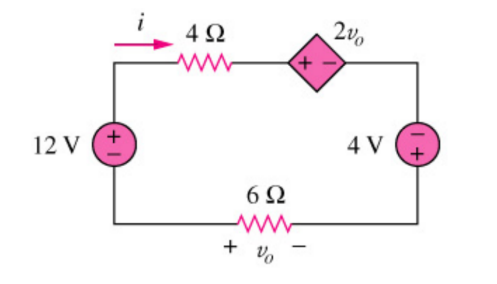
\includegraphics[width=0.5\textwidth]{graphics/ex1/f1.PNG}
    \caption{}
\end{figure}

\subsection{Tính toán}

Áp dụng KVL cho loop theo chiều kim đồng hồ, ta có:
\begin{align}
    -12 + 4i +2v_0 - 4 + 6i = 0
\end{align}
Áp dụng định luật Ohm cho điện trở $6 \Omega$
\begin{align}
    v_0 = -6i
\end{align}
Từ (1.1) và (1.2), ta được:
\begin{align*}
    -16 + 10i - 12i = 0 \rightarrow i = -8 \ \text{A}
\end{align*}
và \(v_0 = 48 \ \text{V}\)

\subsection{Mô phỏng}

Kết quả mô phỏng:

\begin{figure}[!htbp]
    \centering
    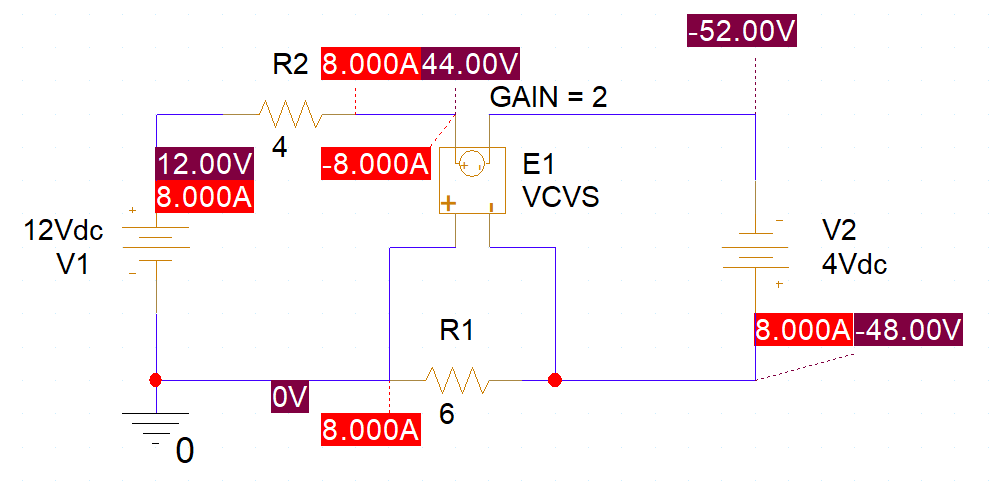
\includegraphics[width=0.7\textwidth]{graphics/ex1/f2.PNG}
\end{figure}
\section{Metal Oxide Semiconductor FET}
As well as the Junction Field Effect Transistor (JFET), there is another type of Field Effect Transistor available whose Gate input is electrically insulated from the main current carrying channel and is therefore called an Insulated Gate Field Effect Transistor.

The most common type of insulated gate FET which is used in many different types of electronic circuits is called the Metal Oxide Semiconductor Field Effect Transistor or MOSFET for short.

The IGFET or MOSFET is a voltage controlled field effect transistor that differs from a JFET in that it has a “Metal Oxide” Gate electrode which is electrically insulated from the main semiconductor n-channel or p-channel by a very thin layer of insulating material usually silicon dioxide, commonly known as glass.
\subsection{Depletion-mode MOSFET}
The Depletion-mode MOSFET, which is less common than the enhancement mode types. This device is very similar to JFET, except that the maximum current saturation is obtained at VGS > 0.  The circuit used to verify IDSS and VP for DFET is presented as follows:
\begin{figure}[!htp]
    \centering
    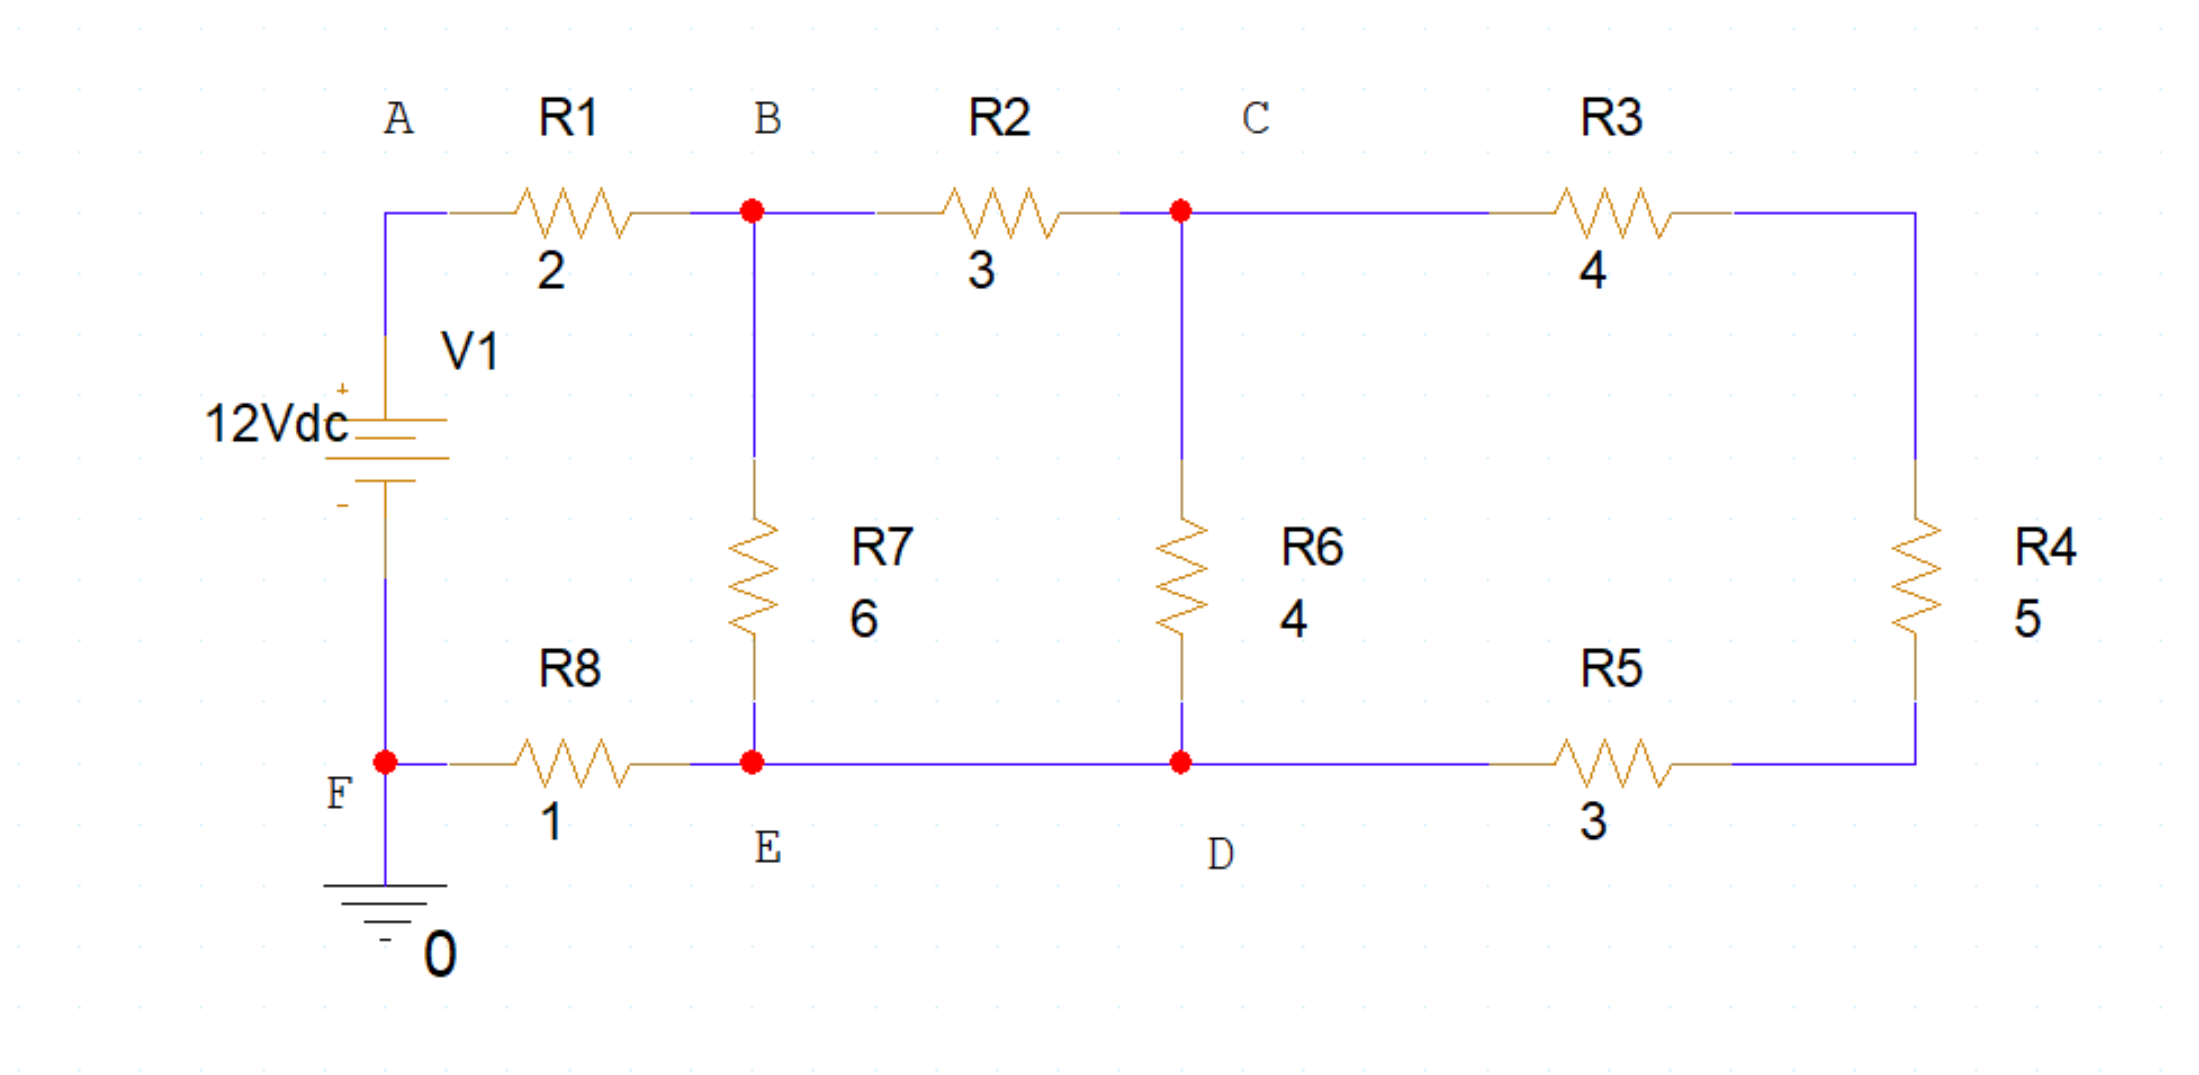
\includegraphics[width = 3in]{graphics/ex2/f1.png}
    \caption{DFET verification in PSPICE}
    \label{dfet_1}
\end{figure}
\pagebreak
The device for a common DFET is MbreakND. After a dc sweep simulation when V3 varies from -5V to 0V, the results are shown bellow:
\begin{figure}[!htp]
    \centering
    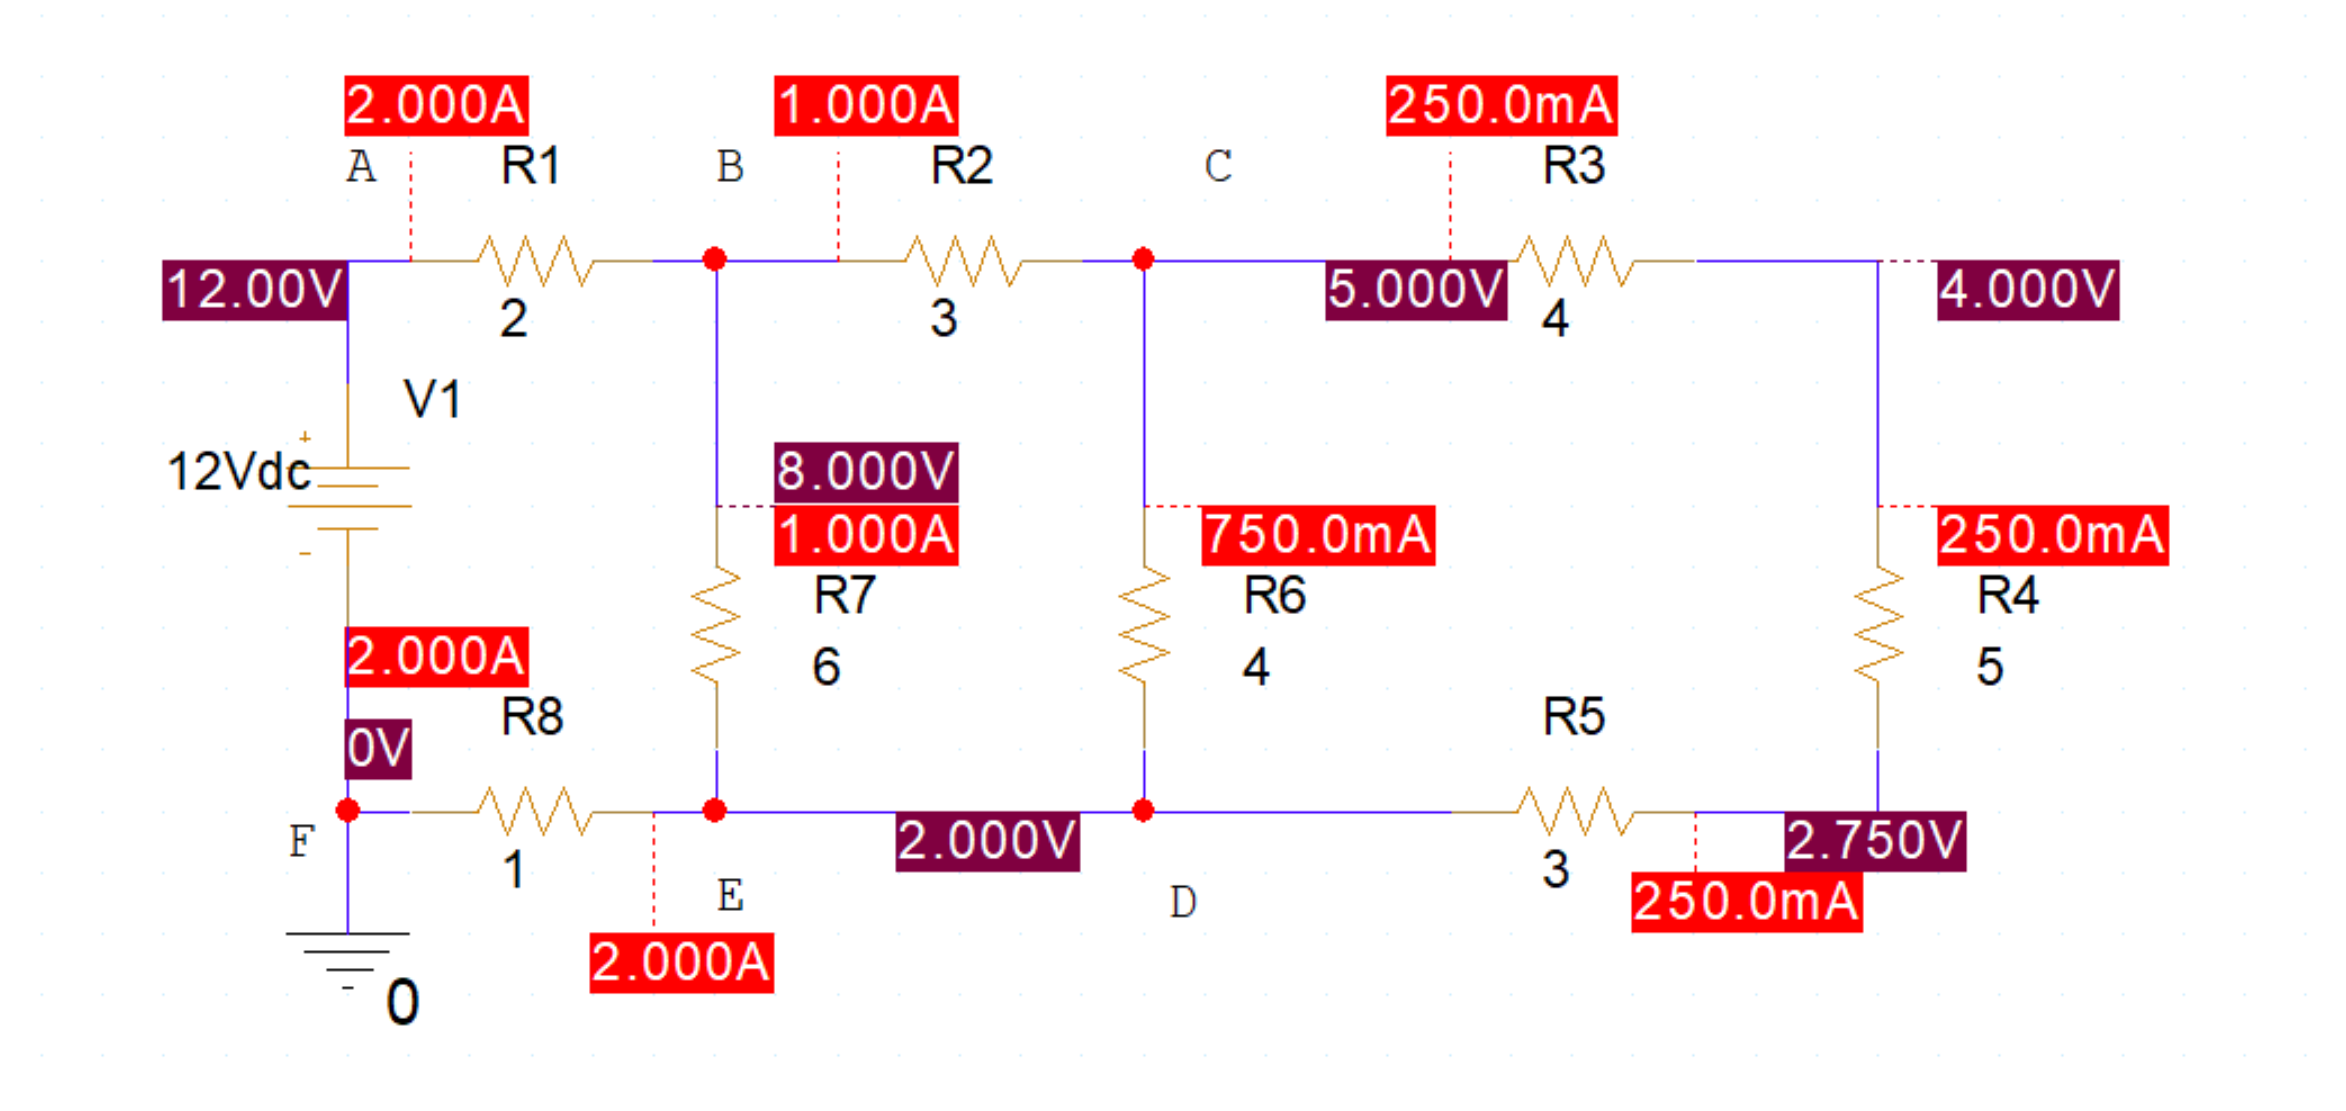
\includegraphics[width = 3in]{graphics/ex2/f2.png}
    \caption{Simulation results with DFET}
    \label{dfet_2}
\end{figure}

From this simulation results, it is confirmed that IDSS = 160mA and VP = -4V for DFET.

\textbf{Students are proposed to implement the circuit bellow:}
\begin{figure}[!htp]
    \centering
    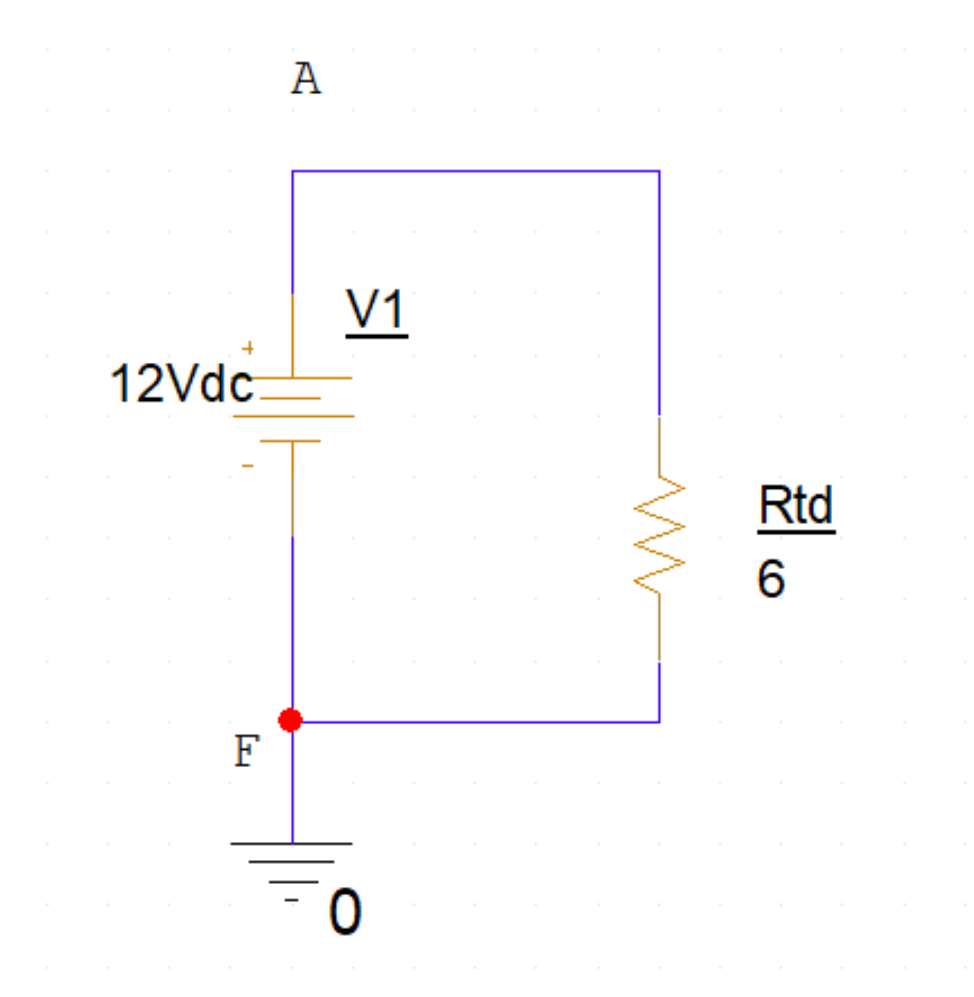
\includegraphics[width = 3in]{graphics/ex2/f3.png}
    \caption{Self bias configuration for DFET}
    \label{dfet_3}
\end{figure}



Only the bias configuration is required to executed. Please capture the simulation results with current and voltage information on the circuit. Finally, explain these values by theory cal-culations.

\textbf{a) Theory Calculation}
\begin{equation}
    I_D = I_{DSS} \left( 1 - \frac{V_{GS}}{V_P} \right)^2 \tag{1}
\end{equation}

\begin{equation}
    V_{GS} = -I_D \cdot R_S \tag{2}
\end{equation}

From equations (1) and (2), we get:
\begin{equation}
    I_D = I_{DSS} \left( 1 - \frac{-I_D \cdot R_S}{V_P} \right)^2
\end{equation}

With:
\[
    I_{DSS} = 160 \, (\mu A), \quad V_P = -4 \, (V), \quad R_S = 1 \, (k\Omega)
\]

Thus:
\[
    I_D = 107.9 \, (mA) \quad (\text{omit } I_D = 148.4 \, (\mu A) \text{due to } \, I_D > I_{DSS})
\]
\[
    V_{GS} = -148.4 \, (mV)
\]
\textbf{b) Pspice Simulation}
\begin{figure}[!htp]
    \centering
    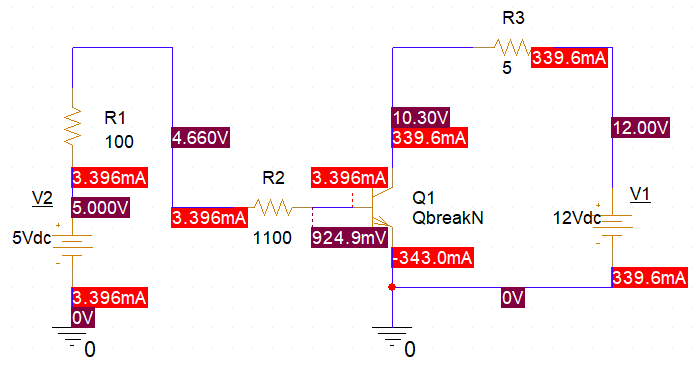
\includegraphics[width=0.5\textwidth]{graphics/ex2/f4.PNG}
\end{figure}

\subsection{Enhancement-mode MOSFET}
The more common Enhancement-mode MOSFET or eMOSFET. The device is normally “OFF” (non-conducting) when the gate bias voltage, VGS is equal to zero. For the n-channel enhance-ment MOS transistor a drain current will only flow when a gate voltage ( VGS ) is applied to the gate terminal greater than the threshold voltage ( VTH ) level in which conductance takes place making it a transconductance device. In other words, for an n-channel enhancement mode MOSFET: +VGS turns the transistor “ON”, while a zero or -VGS turns the transistor “OFF”. Thus the enhancement-mode MOSFET is equivalent to a “normally-open” switch.

The reverse is true for the p-channel enhancement MOS transistor. When VGS = 0 the device is “OFF” and the channel is open. The application of a negative (-ve) gate voltage to the p-type eMOSFET enhances the channels conductivity turning it “ON”. Then for an p-channel enhancement mode MOSFET: +VGS turns the transistor “OFF”, while -VGS turns the transistor “ON”.

The validation of an EFET in PSPICE is presented bellow. The typical EFET in PSPICE is \textbf{MbreakN} device.
\begin{figure}[!htp]
    \centering
    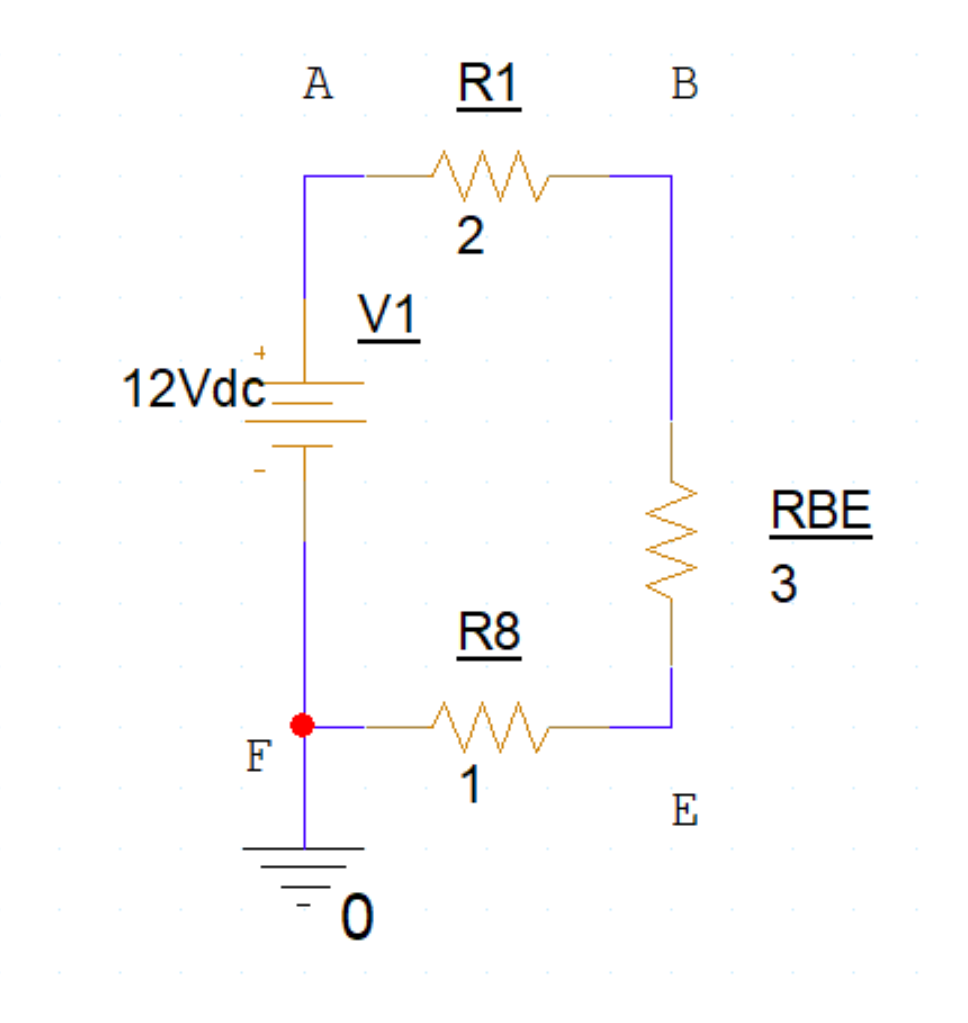
\includegraphics[width = 3in]{graphics/ex2/f5.png}
    \caption{EFET validation}
\end{figure}

A dc sweep simulation with V3 can be performed. The simulation results with V3 varies from -1V to 5V are presented as following:
\begin{figure}[!htp]
    \centering
    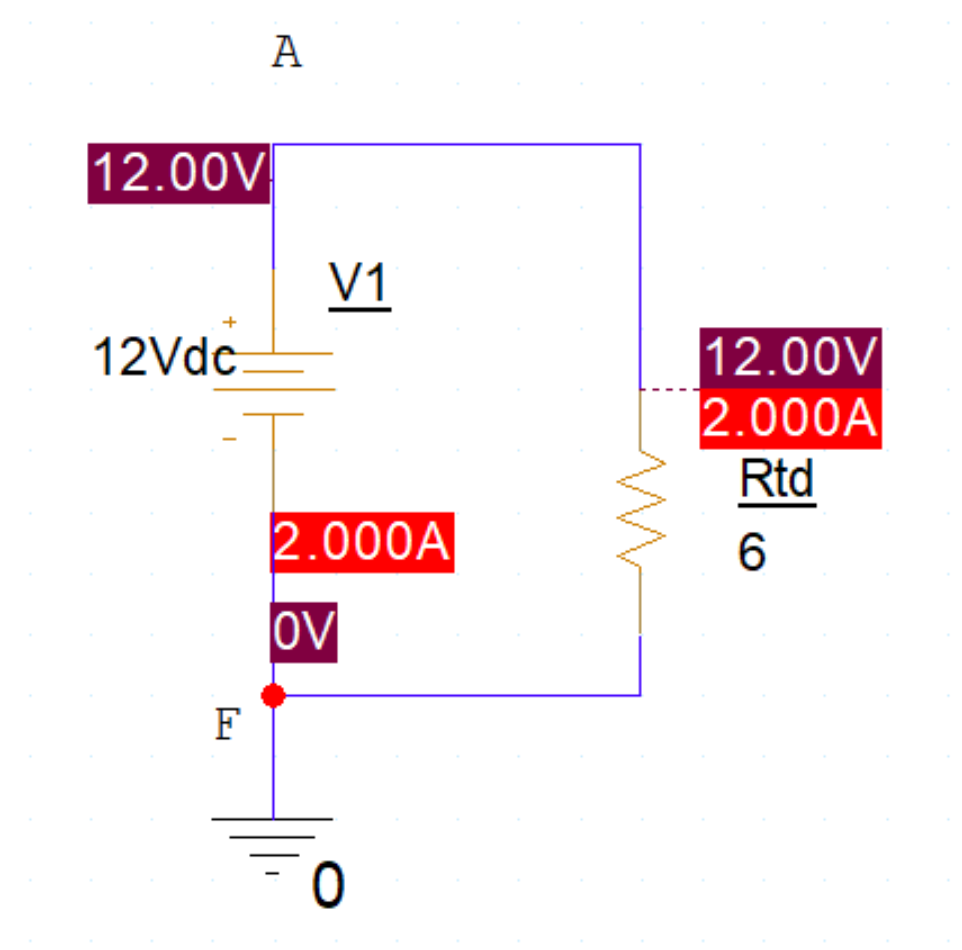
\includegraphics[width = 4.5in]{graphics/ex2/f6.png}
    \caption{Simulation results with EFET}
\end{figure}
\section{Exercise 3}
Cho sơ đồ mạch điện sau, vẽ lại mạch sao cho mạch thể hiện rõ sự nối tiếp và/hoặc song song giữa các điện trở. Sau đó tính điện trở tương đương giữa A và F, điện thế tại A, B, C, D và E. Cuối cùng, sử dụng mô phỏng để kiểm tra phép tính.
\begin{figure}[!htbp]
    \centering
    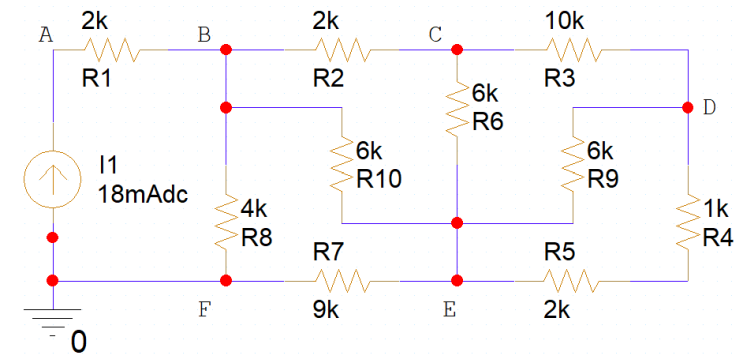
\includegraphics[width=0.7\textwidth]{graphics/ex3/f2.PNG}
    \caption{Mạch ban đầu}
\end{figure}

\subsection{Vẽ lại mạch}

\begin{figure}[!htbp]
    \centering
    \includegraphics[width=1\textwidth]{graphics/ex3/f1.PNG}
    \caption{Mạch tương đương}
\end{figure}

\pagebreak

\subsection{Tính toán}

\begin{align*}
    R_{DE} & = \frac{(R_4 + R_5)R_9}{R_4 + R_5 + R_9} = 2 \text{k}\Omega                            \\
    R_{CE} & = \frac{(R_{DE} + R_3)R_6}{R_{DE} + R_3 + R_6} = 4 \text{k}\Omega                      \\
    R_{BE} & = \frac{(R_{CE} + R_2) R_{10}}{R_{CE} + R_{2} + R_{10}} = 3 \, \text{k}\Omega.         \\
    R_{BF} & = \frac{(R_{BE} + R_{7}) R_{8}}{R_{BE} + R_{7} + R_{8}} = 3 \, \text{k}\Omega.         \\
    R_{AF} & = R_{1} + R_{BF} = 5 \, \text{k}\Omega.                                                \\ \\
%
    V_{AF} & = R_{AF} I_1 = 90 \, \text{V}.                                                         \\
    V_{BF} & = R_{BF}I_1 = 54 \, \text{V}.                                                          \\
    V_{EF} & = \frac{R_{7}}{R_{BE} + R_{7}} V_{BF} = 40.5 \, \text{V}.                               \\
    V_{BE} & = V_{BF} - V_{EF} = 13.5 \, \text{V}.                                                        \\
    V_{CF} & = \frac{R_{CE}}{R_{2} + R_{CE}} V_{BE} + V_{EF} = 49.5 \, \text{V}.                             \\
    V_{DF} & = \frac{R_{DE}}{R_{DE} + R_{3}} \frac{R_{CE}}{R_{2} + R_{CE}} V_{BE} + V_{EF} = 42 \, \text{V}. \\
\end{align*}
%
Cho \(V_F = 0\)
%
\begin{align*}
    V_{A} & = 90 \, \text{V}.   \\
    V_{B} & = 54 \, \text{V}.   \\
    V_{C} & = 49.5 \, \text{V}. \\
    V_{D} & = 42 \, \text{V}.   \\
    V_{E} & = 40.5 \, \text{V}. \\
\end{align*}

\pagebreak

\subsection{Mô phỏng}

\begin{figure}[!htbp]
    \centering
    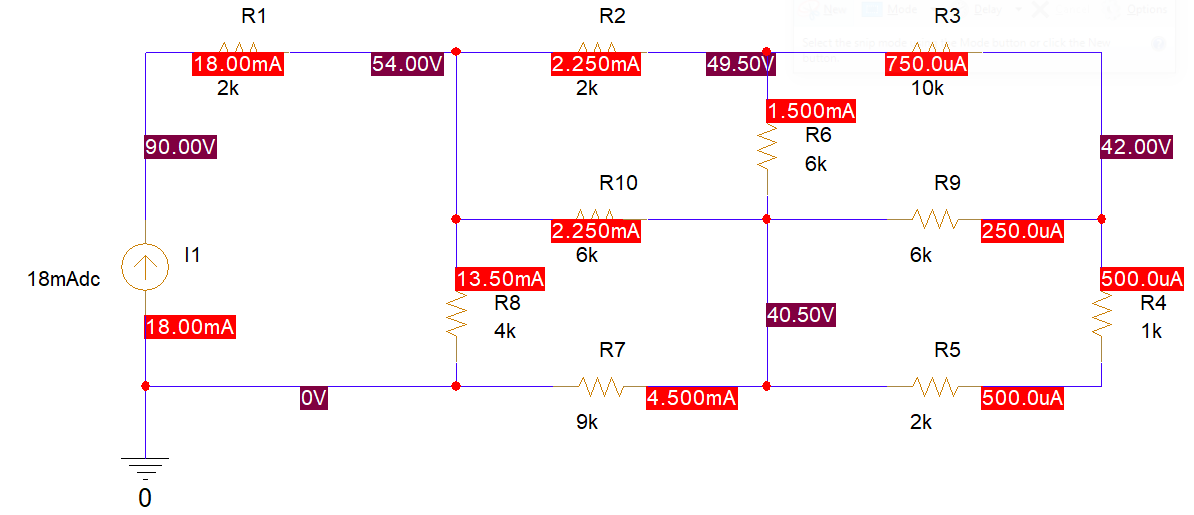
\includegraphics[width=1\textwidth]{graphics/ex3/f3.PNG}
    \caption{Mạch ban đầu}
    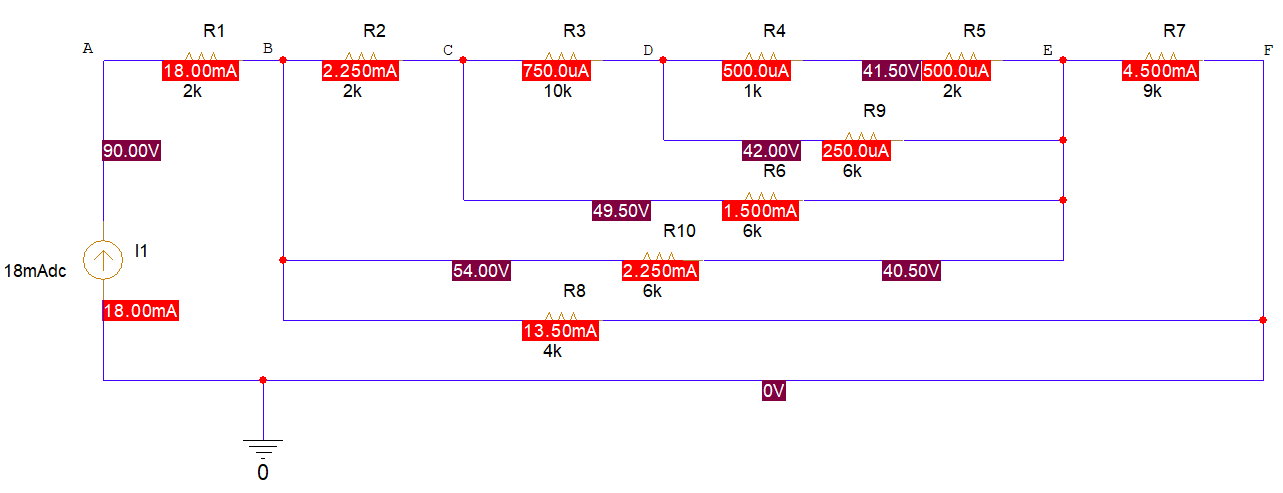
\includegraphics[width=1\textwidth]{graphics/ex3/f4.PNG}
    \caption{Mạch tương đương}
\end{figure}


\section{Clamper Diode Circuit}

Các mạch trong hình bên dưới được gọi là bộ kẹp hoặc bộ phục hồi DC. Mô phỏng trên PSpice cũng được hiển thị trong hình bên dưới. Các mạch này kẹp một đỉnh của dạng sóng ở mức DC cụ thể (ví dụ: 0,7V). Học sinh được yêu cầu triển khai mạch trong PSPice để xác minh kết quả của họ từ tính toán lý thuyết.

\begin{figure}[h]
    \centering
    \includegraphics[width=0.5\textwidth]{graphics/ex4/f1.PNG}
    \caption{Mạch kẹp sử dụng Diode}
\end{figure}

\subsection{Tính toán lý thuyết}

Trong phần này, giả định rằng mô hình diode thực tế được sử dụng. Trình bày các phương trình của bạn để tính toán ba dòng điện khác nhau, bao gồm $I_{R1}, I_{R2}, I_{D2}$ và điện áp $V_{R2}$.

Theo Kirchhoff’s Voltage Law (KVL), ta có hai phương trình sau:
\begin{align}
    &E - V_{D1} - V_{D2} - 5.6 \cdot I_{R1} = 0 \\
    &V_{D2} = 3.3 \cdot I_{R2}
\end{align}
Theo Kirchhoff’s Current Law (KCL), ta có:
\begin{align}
    I_{R1} &= I_{R2} + I_{D2}
\end{align}

Từ (3.1), (3.2) và (3.3), ta có:
\begin{align*}
    &I_{R1} = 3,321 \, \text{mA} \\
    &I_{R2} = 0,212 \, \text{mA} \\
    &I_{D2} = 3,109 \, \text{mA} \\
    &V_{R2} = V_{D2} = 0.7 \, \text{V}
\end{align*}

\subsection{Mô phỏng PSpice}

Mô phỏng bias point được chạy trong PSpice. Chụp màn hình của bạn với điện áp và dòng điện được bật trong kết quả.

\begin{figure}[h]
    \centering
    \begin{subfigure}{0.49\textwidth}
        \centering
        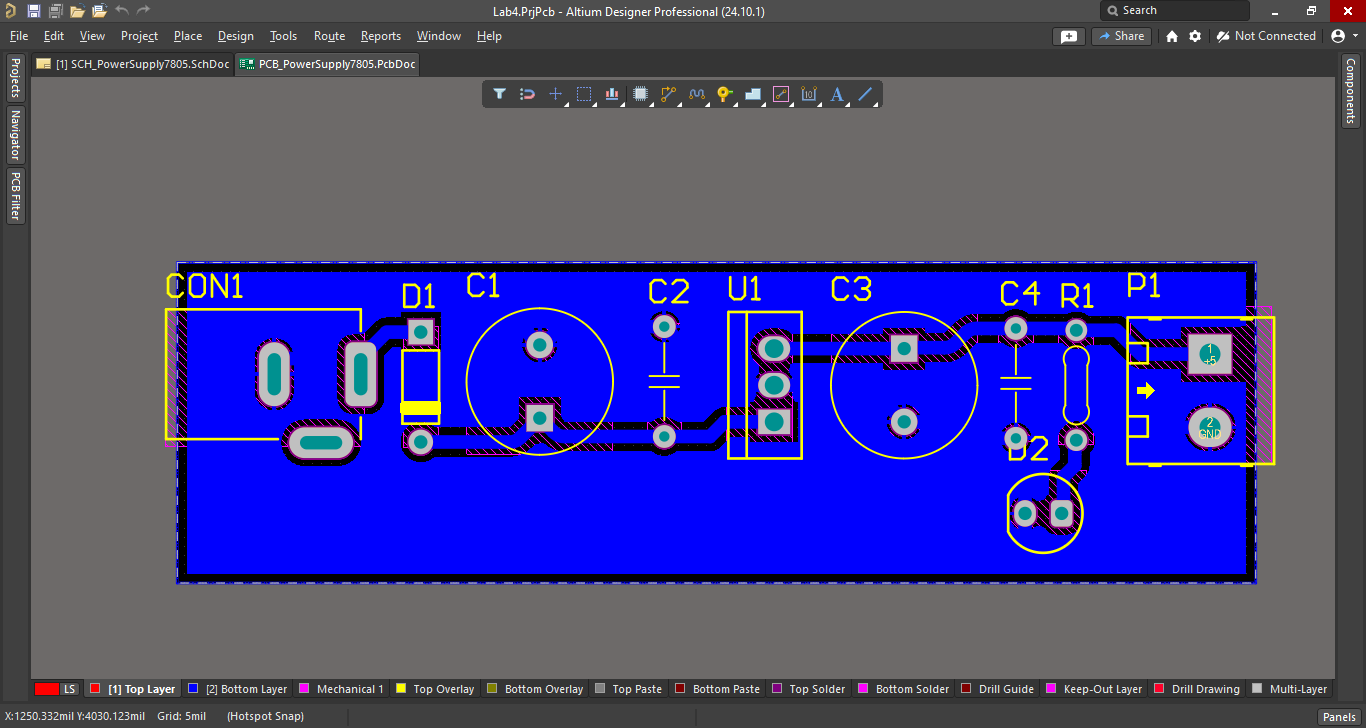
\includegraphics[width=\linewidth]{graphics/ex4/f2.PNG}
    \end{subfigure}
    \hfill
    \begin{subfigure}{0.49\textwidth}
        \centering
        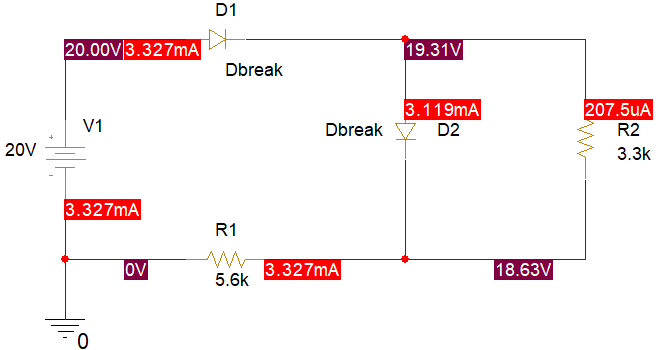
\includegraphics[width=\linewidth]{graphics/ex4/f3.PNG}
    \end{subfigure}
    \caption{Kết quả mô phỏng trên PSpice}
\end{figure}

\subsection{So sánh}

Sinh viên phải tóm tắt kết quả từ cả tính toán lý thuyết và mô phỏng PSpice và điền vào bảng bên dưới.

\begin{table}[h]
    \centering
    \begin{tabular}{@{}lcccccccc@{}}
        \toprule
        & \multicolumn{4}{c}{\textbf{Theory calculation}} & \multicolumn{4}{c}{\textbf{PSpice simulation}} \\

        \cmidrule(rl{0.5cm}){2-5} \cmidrule(rl{0.5cm}){6-9}

        & \makecell{\(I_{R1}\) \\(mA)} & \makecell{\(I_{R2}\) \\ (mA)} & \makecell{\(I_{D2}\) \\ (mA)} & \makecell{\(V_{R2}\) \\ (V)} & \makecell{\(I_{R1}\) \\ (mA)} & \makecell{\(I_{R2}\) \\ (mA)} & \makecell{\(I_{D2}\) \\ (mA)} & \makecell{\(V_{R2}\) \\ (V)} \\

        \midrule

        \(V\) = 12V & 1.893 & 0.212 & 1.681 & 0.70 & 1.903 & 0.203 & 1.701 & 0.67 \\
        \(V\) = 20V & 3.321 & 0.212 & 3.109 & 0.70 & 3.327 & 0.208 & 3.119 & 0.68 \\

        \bottomrule
    \end{tabular}
\end{table}

\textbf{Kết luận:} Chúng ta có thể thấy rằng với mạch này, trong mô hình Practical diode, diode D2 cố định điện áp và dòng điện qua R2, ở mọi giá trị của V. Ngược lại, trong mô phỏng Pspice, do điện trở nội bên trong Diode không phải là hằng số nên hai giá trị trên có sự khác nhau ở hai trường hợp.
\section{Power switching circuit}

Sự sập nguồn điện chính có thể rất quan trọng trong nhiều tình huống khác nhau. Ví dụ, khi nguồn điện bị mất đột ngột, bạn có thể muốn lưu một số dữ liệu dự phòng trên vi điều khiển. Những trường hợp như vậy cần một số mạch chuyển đổi tự động sang nguồn điện dự phòng, chẳng hạn như pin.

\begin{figure}[H]
    \centering
    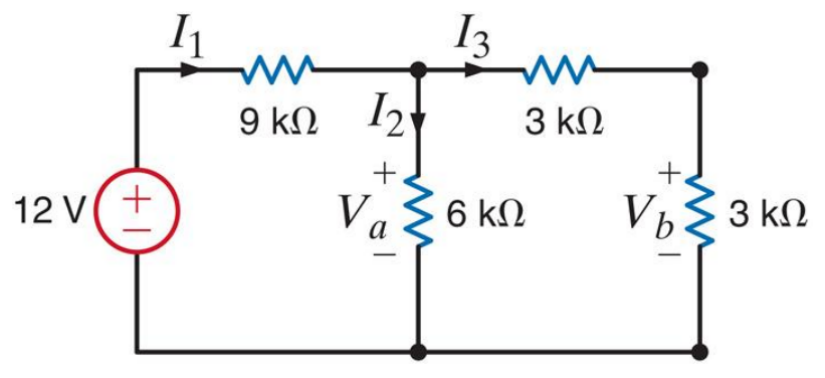
\includegraphics[width=0.8\textwidth]{graphics/ex5/f1.png}
    \caption{Mạch chuyển nguồn điện}
\end{figure}
Giải pháp đơn giản nhất cho vấn đề này là thêm một diode vào mỗi nguồn điện, như được hiển thị trong hình trên. Trong mạch này, nguồn điện 5V được sử dụng là một pin dự phòng. Trong khi đó, 9V là nguồn điện chính cho hệ thống, được minh họa bằng một điện trở tải.


Tuy nhiên, vấn đề của cách tiếp cận có phần ngây thơ này là sự sụt áp (phân cực thuận) qua diode có thể quá cao đối với hệ thống. Nhờ vào diode Schottky, điều này có thể được giảm thiểu bằng cách sử dụng loại có điện áp thuận cực thấp, có thể tìm thấy trên thị trường (ví dụ: diode Schottky sụt áp khoảng 250mV tại 1A).

\subsection{Tính toán theo lý thuyết}
\subsubsection{Trường hợp chỉ có nguồn 5V}
Dễ thấy D4 là diode phân cực nghịch nên không dẫn điện. Do đó, \(I_{D4} = 0\). Các đại lượng còn lại được tính như sau:
\begin{align*}
I_{D3} &= \frac{5V - V_{D3}}{R_{L}} = \frac{5V - 0.7V}{1k\Omega} = 4.3mA  \\
% I_{D4} &= 0 \\
I_{RL} &= I_{D3} = 4.3mA \\
V_{RL} &= I_{RL} \times R_{L} = 4.3mA \times 1k\Omega = 4.3V
\end{align*}

\subsubsection{Trường hợp chỉ có nguồn 9V}
Dễ thấy D3 là diode phân cực nghịch nên không dẫn điện. Do đó, \(I_{D3} = 0\). Các đại lượng còn lại được tính như sau:
\begin{align*}
% I_{D3} &= 0 \\
I_{D4} &= \frac{9V - V_{D4}}{R_{L}} = \frac{9V - 0.7V}{1k\Omega} = 8.3mA\\
I_{RL} &= I_{D4} = 8.3mA \\
V_{RL} &= I_{RL} \times R_{L} = 8.3mA \times 1k\Omega = 8.3V
\end{align*}

\subsubsection{Trường hợp có cả nguồn 5V và nguồn 9V}
Trường hợp này ta thấy D4 là diode phân cực thuận, D3 là diode phân cực nghịch nên không dẫn điện, \(I_{3} = 0V\). Các đại lượng còn lại được tính như sau:
\begin{align*}
% I_{D3} &= \frac{5V - V_{D3}}{R_{L}} \\
I_{D4} &= \frac{9V - V_{D4}}{R_{L}} = \frac{9V - 0.7V}{1k\Omega} = 8.3mA\\
I_{RL} &= I_{D4} = 8.3mA \\
V_{RL} &= I_{RL} \times R_{L} = 8.3mA \times 1k\Omega = 8.3V
\end{align*}

\subsection{Mô phỏng PSpice}
\begin{figure}[H]
    \centering
    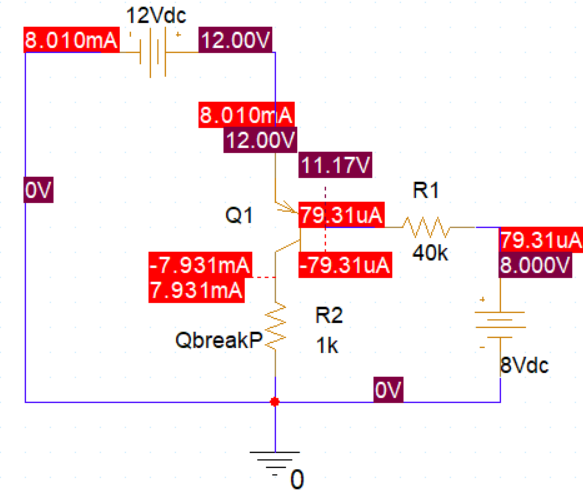
\includegraphics[width=1\textwidth]{graphics/ex5/f2.png}
    \caption{Trường hợp chỉ có nguồn 5V}
\end{figure}

\begin{figure}[H]
    \centering
    \includegraphics[width=1\textwidth]{graphics/ex5/f3.png}
    \caption{Trường hợp chỉ có nguồn 9V}
\end{figure}

\begin{figure}[H]
    \centering
    \includegraphics[width=1\textwidth]{graphics/ex5/f4.png}
    \caption{Trường hợp có cả nguồn 5V và nguồn 9V}
\end{figure}

\subsection{So sánh}
\begin{table}[H]
    \centering
    \begin{tabular}{|c|c|c|c|c|c|c|c|c|}
        \cline{2-9}
        \multicolumn{1}{c|}{} & \multicolumn{4}{c|}{\textbf{Tính toán theo lý thuyết}} & \multicolumn{4}{c|}{\textbf{Mô phỏng PSpice}} \\ \cline{2-9}
        \multicolumn{1}{c|}{} & \(I_{D3}\) & \(I_{D4}\) & \(I_{RL}\) & \(V_{RL}\) & \(I_{D3}\) & \(I_{D4}\) & \(I_{RL}\) & \(V_{RL}\) \\ \hline
        \textbf{Chỉ 5V} & 4.3mA & 0A & 4.3mA & 4.3V & 4.307mA & 4.317pA & 4.307mA & 4.307V \\ \hline
        \textbf{Chỉ 9V} & 0A & 8.3mA & 8.3mA & 8.3V & 8.299pA & 8.289mA & 8.289mA & 8.289V \\ \hline
        \textbf{5V và 9V} & 0A & 8.3mA & 8.3A & 8.3V & 8.299pA & 8.289mA & 8.289mA & 8.289V \\ \hline
    \end{tabular}
\end{table}

Chức năng cuối cùng của các diode trong mạch này là bảo vệ mạch khỏi dòng điện ngược chiều trong trường hợp cả hai nguồn được bật cùng lúc. Trường hợp này rất phổ biến khi vi điều khiển được lập trình và cấp nguồn bởi đồng thời cổng USB và nguồn điện bên ngoài.
\section{PNP Circuit}
Figure \ref{lab3_ex6_de} shows a very typical PNP transistor circuit.
Calculate $I_B$, $I_E$, and $I_C$ then simulate the circuit to double-check your calculation. Assume the current gain $\beta$ = 100.

\begin{figure}[H]
    \centering
    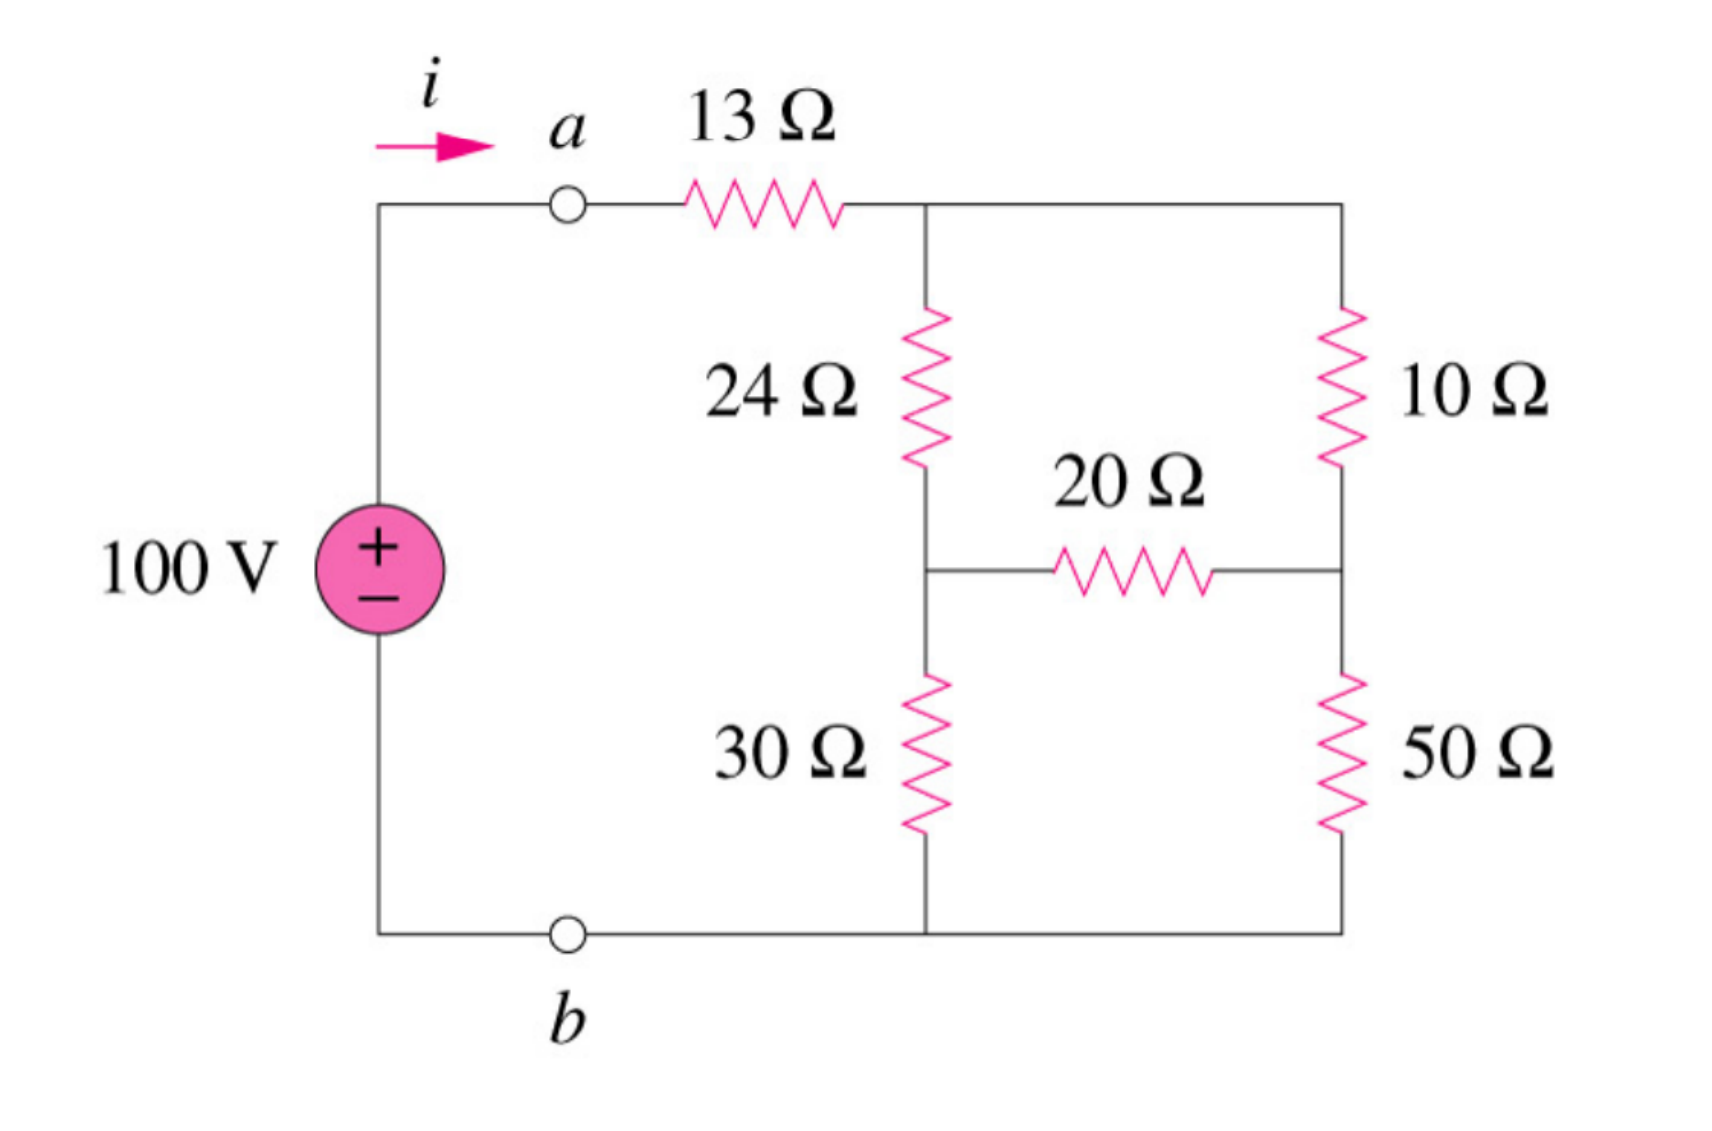
\includegraphics[width=0.5\linewidth]{graphics/ex6/f1.png}
    \caption{A PNP Circuit}
    \label{lab3_ex6_de}
\end{figure}

\subsection{Theoretical calculation}
\textit{\textbf{Notes:}}\\
\textit{Explanations, formulas, and equations are expected rather than only results.}

\begin{itemize}
    \item Vì đây là PNP transistor, nên $V_{EB}$ = 0.7 V (tránh nhầm lẫn với $V_{BE}$ trong NPN transistor).
    \item Áp dụng KVL: $$V_{EE} - V_{BB} - V_{EB} = I_B \times R_B $$
    $$ => I_B = \frac{V_{EE} - V_{BB} - V_{EB}}{R_B} = \frac{12V - 8V - 0.7V}{40k \Omega} = 82.5 \mu A $$
    \item $I_C = \beta \times I_B = 100 \times 82.5 \mu A = 8.25 mA $
    \item $I_E = I_B + I_C = 82.5\mu A + 8.25mA = 8.3325 mA$
\end{itemize}

\subsection{Simulation}
% \textbf{\textit{Your image goes here}}
\begin{figure}[H]
    \centering
    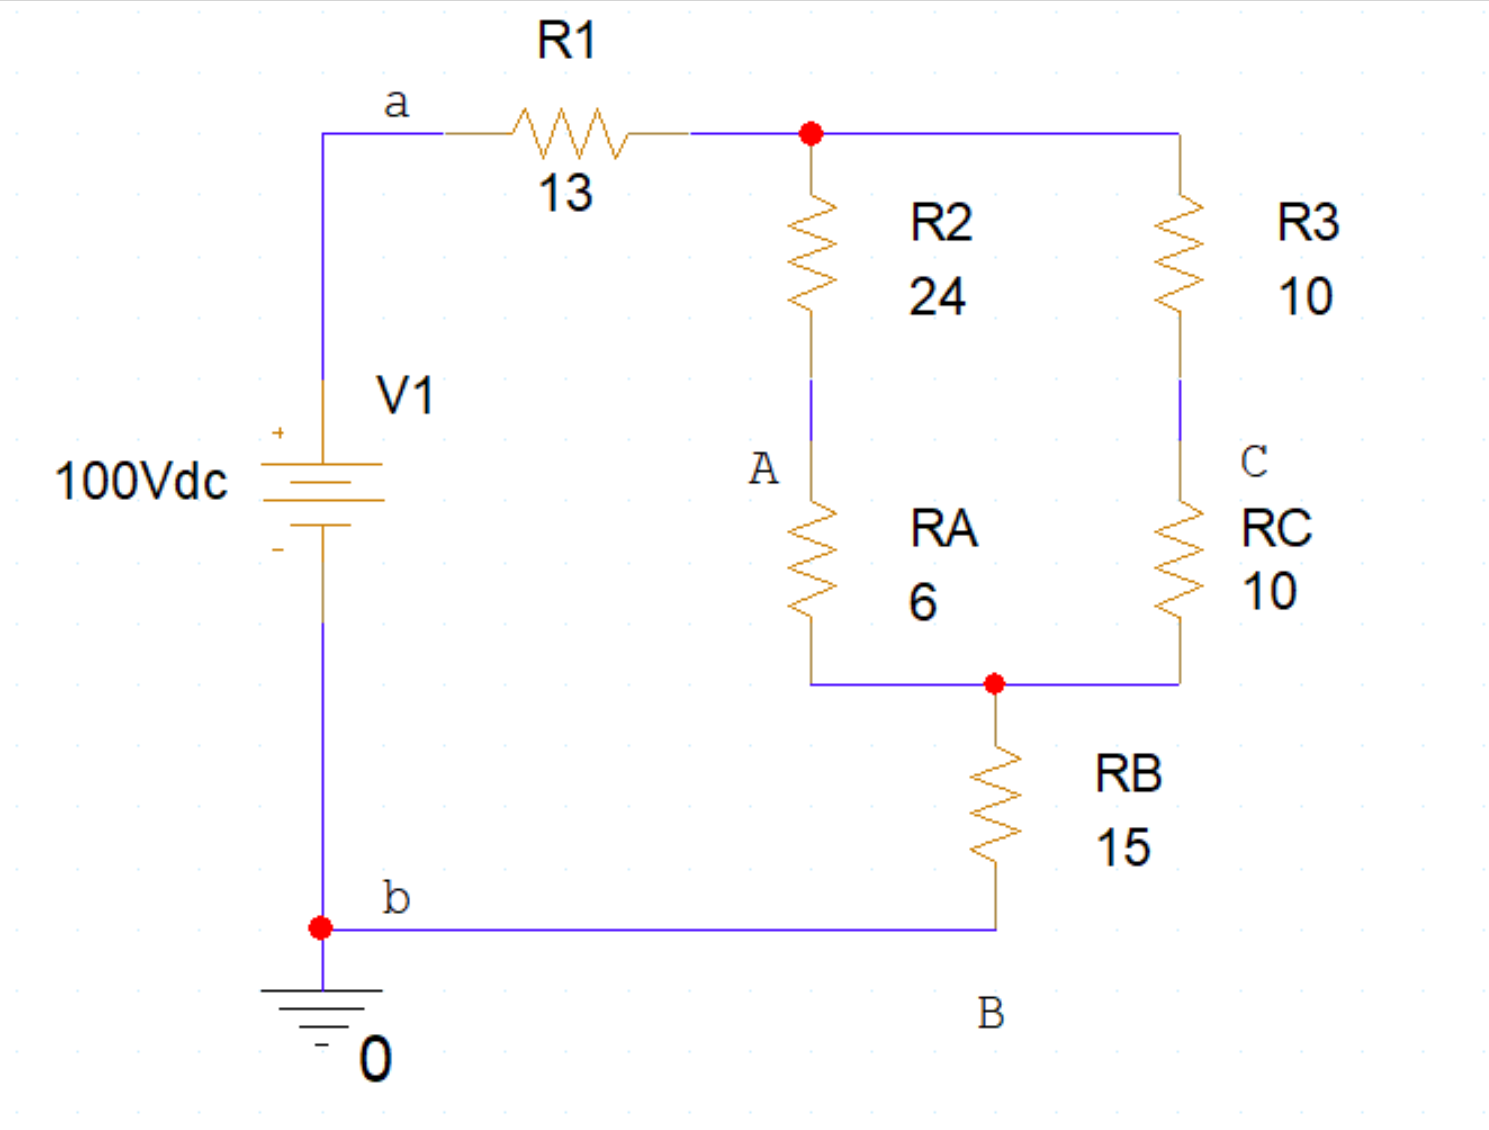
\includegraphics[width=0.9\linewidth]{graphics/ex6/f2.png}
    % \caption{A PNP Circuit}
\end{figure}

\subsection{Comparison}
$I_B$ (lý thuyết) = \dotfill$82.5 \mu A$ \dotfill $I_B$ (mô phỏng) =\dotfill $79.31 \mu A$\dotfill\bigskip\\
$I_C$ (lý thuyết) = \dotfill$ 8.250 mA$\dotfill $I_C$ (mô phỏng) = \dotfill $7.931mA$\dotfill\bigskip\\
$I_E$ (lý thuyết) = \dotfill$8.3325 mA$\dotfill $I_E$ (mô phỏng) = \dotfill$8.010mA $\dotfill\bigskip\\

\section{Exercise 7}
Cho mạch điện như hình. Dựa vào kiến thức đã học, hãy vẽ lại mạch sao cho dễ tính điện trở tương đương \(R_{eq}\). Tiếp theo, tìm giá trị dòng điện \(I_S\) qua mạch và kiểm tra bằng mô phỏng.
\begin{figure}[!htbp]
    \centering
    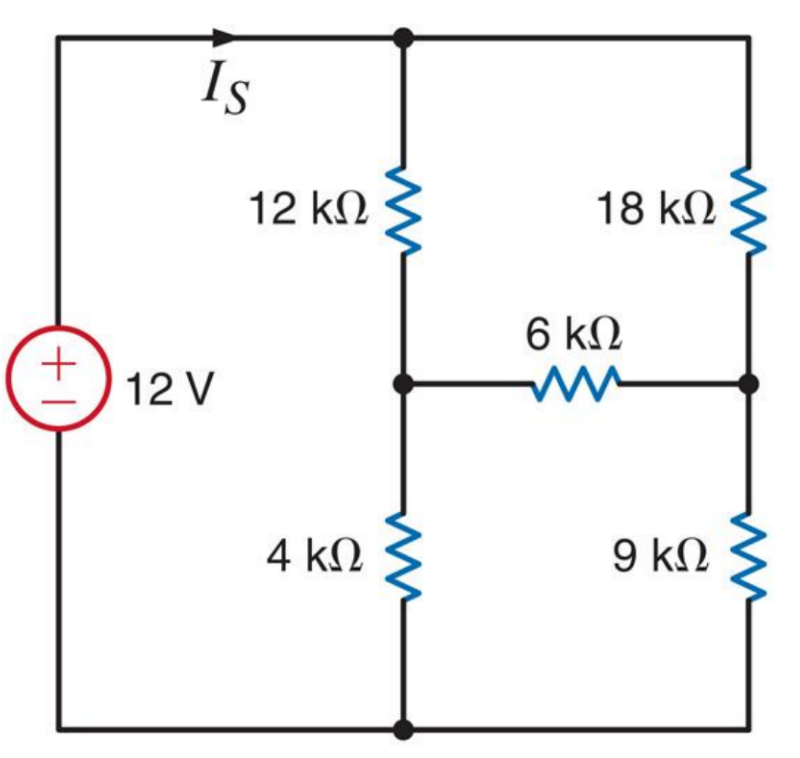
\includegraphics[width=0.7\textwidth]{graphics/ex7/f1.png}
    \caption{Mạch ban đầu}
\end{figure}
\subsection{Biến đổi mạch}
Dễ thấy 3 điện trở \(12k\Omega\), \(18k\Omega\) và \(6k\Omega\) tạo thành mạch \(\Delta\), nên để dễ tính toán hơn thì ta sẽ biến đổi đoạn mạch này về mạch Wye. Cụ thể như hình 7.2.
\begin{figure}[!htbp]
    \centering
    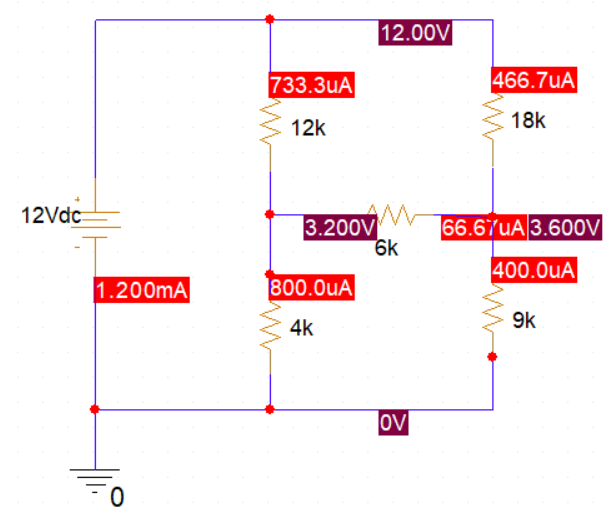
\includegraphics[width=0.7\textwidth]{graphics/ex7/f2.png}
    \caption{Mạch sau khi biến đổi}
\end{figure}
\begin{itemize}
    \item Ta quy ước tên các điện trở trong mạch ban đầu như sau: \(R_a = 6k\Omega,  R_b = 12k\Omega,  R_c = 18k\Omega\).
    \newpage
    \item Tên các điện trở trong mạch sau khi biến đổi được ký hiệu trong hình. Các điện trở mới có giá trị là:
    
    \(R_1 = \frac{R_b \cdot R_c}{R_a + R_b + R_c} = \frac{12k\Omega \cdot 18k\Omega}{6k\Omega + 12k\Omega + 18k\Omega} = 6k\Omega\)

    \(R_2 = \frac{R_a \cdot R_b}{R_a + R_b + R_c} = \frac{6k\Omega \cdot 12k\Omega}{6k\Omega + 12k\Omega + 18k\Omega} = 2 k\Omega\)

    \(R_3 = \frac{R_c \cdot R_a}{R_a + R_b + R_c} = \frac{18k\Omega \cdot 16k\Omega}{6k\Omega + 12k\Omega + 18k\Omega} = 3k\Omega\)
    
\end{itemize}
\subsection{Tính toán}
\begin{itemize}
    \item Sau khi biến đổi, ta dễ dàng tính được điện trở tương đương của mạch:
    
    \(R_{eq} = 6k\Omega + \frac{(3k\Omega + 9k\Omega) \cdot (2k\Omega + 4k\Omega) }{(3k\Omega + 9k\Omega) + (2k\Omega + 4k\Omega)} = 10k\Omega\)
    \item Giá trị dòng điện \(I_S\):
    
    \(I_S = \frac{12V}{R_{eq}} = \frac{12V}{10k\Omega} = 1.2 mA\)

\end{itemize}
\newpage
\subsection{Mô phỏng}
Kết quả mô phỏng:
\begin{figure}[!htbp]
    \centering
    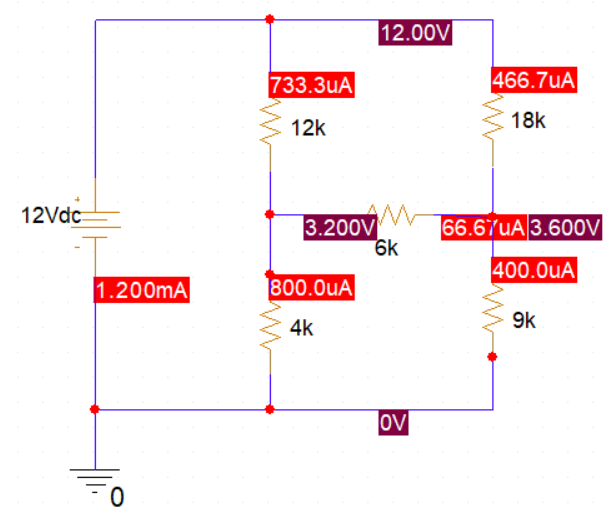
\includegraphics[width=0.7\textwidth]{graphics/ex7/f3.png}
    \caption{Mô phỏng mạch ban đầu}
\end{figure}
\begin{figure}[!htbp]
    \centering
    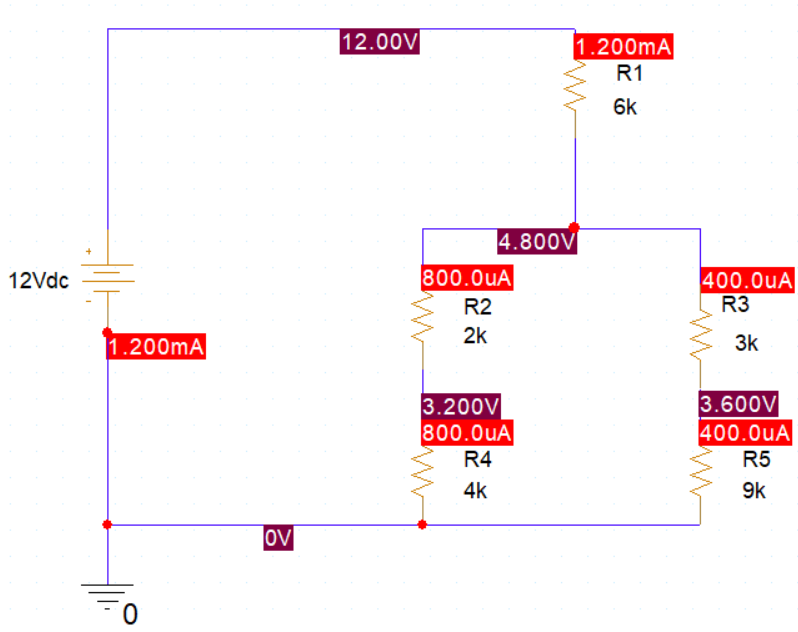
\includegraphics[width=0.7\textwidth]{graphics/ex7/f4.png}
    \caption{Mô phỏng mạch sau khi biến đổi}
\end{figure}
\section{NPN Circuit with E resistance}
In Figure \ref{lab3_ex9_de}, calculate all the values of $I_B$, $I_C$, $I_E$, $V_E$, and $V_C$. Assume the voltage drop $V_{BE}$ = 0.7V and the current gain coefficient of the transistor is $\beta$ = 100. Then, perform a simulation to double-check your theoretical calculations.

\begin{figure}[h]
    \centering
    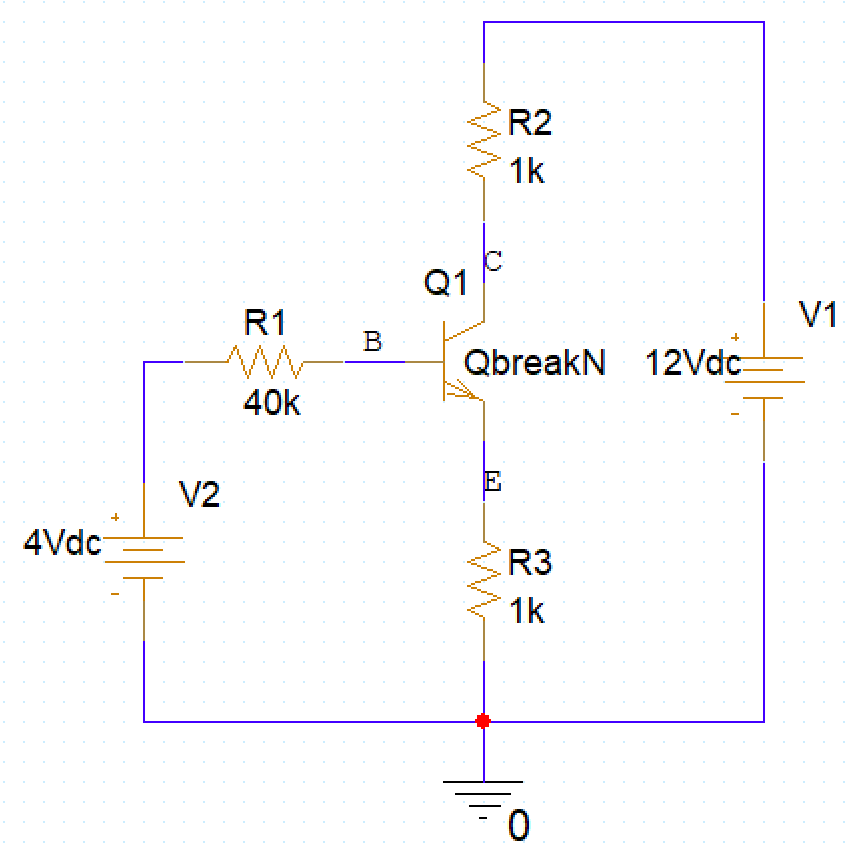
\includegraphics[width=10cm]{graphics/ex8/lab3_ex9_de.png}
    \caption{NPN Circuit with E resistance}
    \label{lab3_ex9_de}
\end{figure}

\subsection{Theoretical calculation}
Note:

Explanations, formulas, and equations are expected rather than only results.

Theo KVL, KCL, định luật Ohm, ta có các phương trình sau:
\[
40000 \cdot I_B + V_{BE} + 1000 \cdot I_E = V_2
\]
\[
\Leftrightarrow 40000 \cdot I_B + V_{BE} + 1000(\beta + 1) \cdot I_B = V_2 \quad (1)
\]
Giải (1), ta có: 
\[
I_B = \frac{V_2 - V_{BE}}{41000 + 1000 \cdot \beta} = 23.4 \, \mu \text{A}
\]
\[
I_C = \beta \cdot I_B = 2.34 \, \text{mA}
\]
\[
I_E = (\beta + 1) \cdot I_B = 2.36 \, \text{mA}
\]
\[
V_E = I_E \cdot R_3 = 2.36 \, \text{V}
\]
\[
V_C = V_1 - I_C \cdot R_2 = 9.66 \, \text{V}
\]

\subsection{Simulation}
Your image goes here
\begin{figure}[h]
    \centering
    \includegraphics[width=0.5\textwidth]{graphics/ex8/f1.PNG}
\end{figure}
\section{Excercise 9}
Cho mạch sau. Tìm điện áp \(v\) và dòng điện \(i_x\) . Theo kết quả, xác định các linh kiện có khả năng hấp thụ lần lượt là p1 và p2 là hoạt động hoặc
thụ động (cần tính toán). Lưu ý rằng ở đây chúng tôi sử dụng quy ước ký hiệu thụ động.
Nếu một phần tử tiêu thụ điện năng, hãy sử dụng điện trở thuần có giá trị phù hợp làm đại diện. Nếu là bộ phận cấp nguồn, hãy sử dụng nguồn điện áp DC lý tưởng tương ứng để
đại diện cho nó. Thực hiện mô phỏng để kiểm tra mạch hoạt động như thế nào.
\begin{figure}[!htbp]
    \centering
    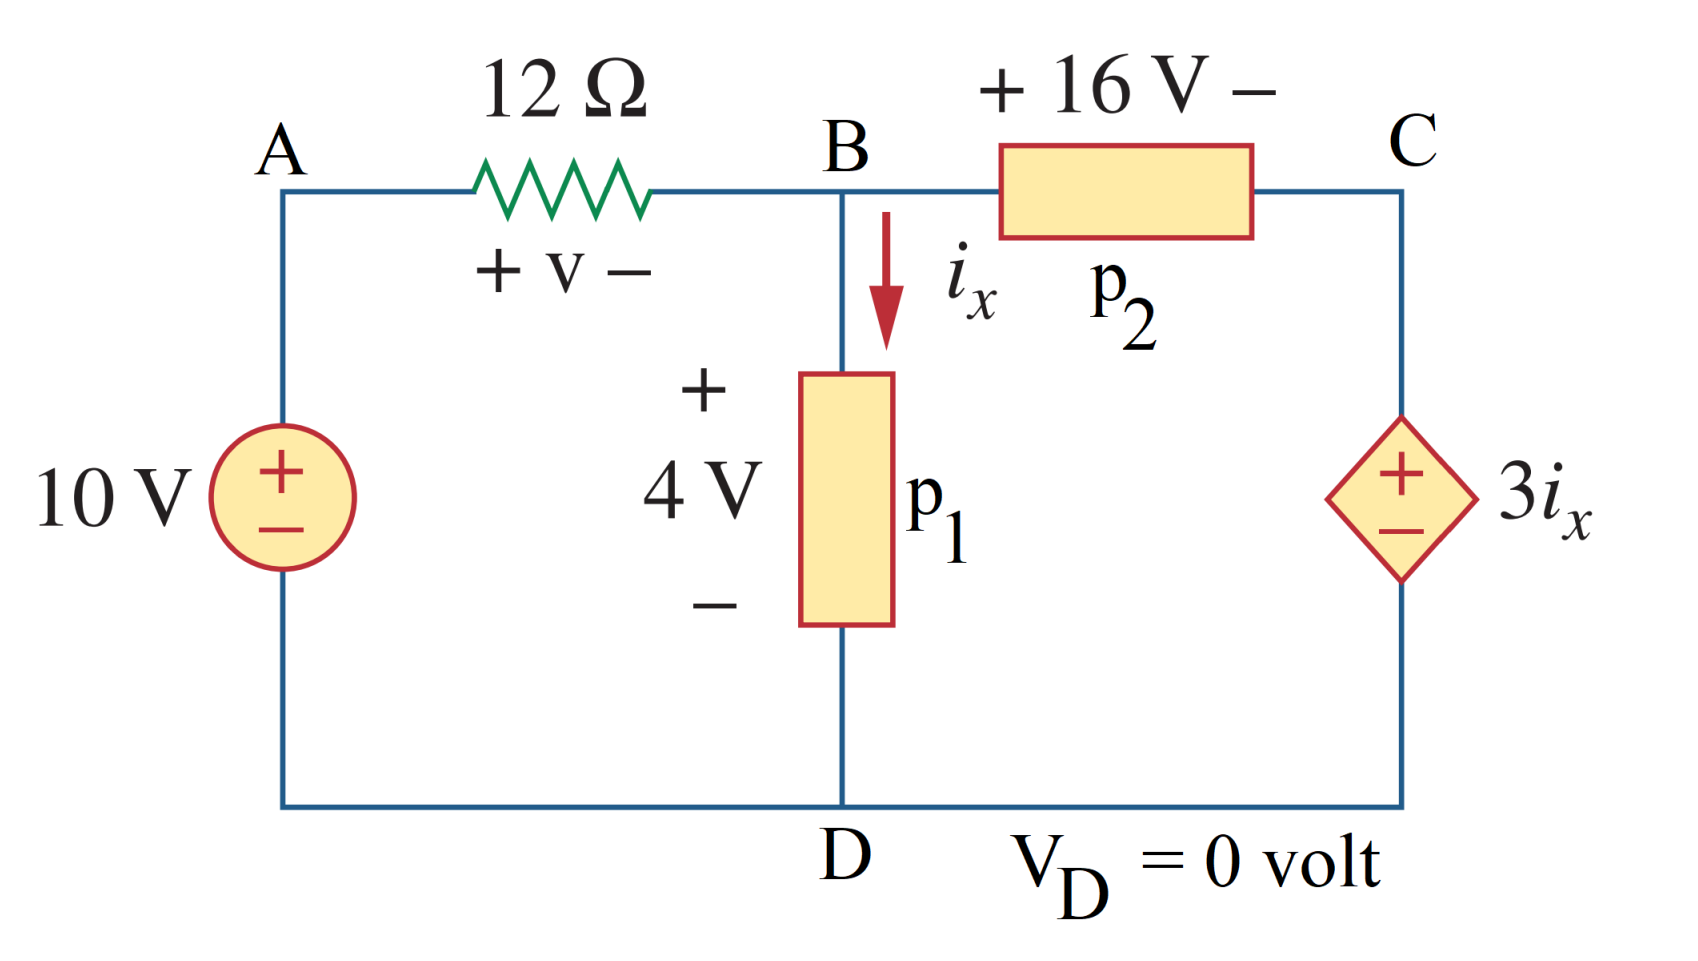
\includegraphics[width=0.7\textwidth]{graphics/ex9/f1.png}
    \caption{Tìm các phần tử và biến chưa biết, sau đó kiểm tra chúng bằng mô phỏng}
    \end{figure}
\subsection{Tính toán}
\textbf{Ghi chú:}
Giải thích, công thức và phương trình được mong đợi hơn là chỉ có kết quả.\\
Theo phân tích lưới.\\
Vòng 1:
\begin{align*}
12I_{AB} + 4 - 10 = 0 \rightarrow I_{AB} = 0,5 (A).
\end{align*}
Vòng 2:
\begin{align*}
    -4 + 16 + 3i_x = 0 \rightarrow i_x = -4 (A).
\end{align*}
Ta có:
\begin{align*}
    v = I_AB.12 =6 (V)\\
    i_x = -4 (A).
\end{align*}

\section{\large AC/DC Power Circuit Application With LM2596\_5P0\_TRANS}
Hình 10.1 mô tả mạch cấp nguồn chuyển mạch LM2596 - 5.0 của Texas Instrument chưa hoàn chỉnh. Nó thiếu bộ điều chỉnh điện áp diode Zener và cuộn cảm giảm điện áp
biến thể. Đầu tiên, hãy thực hiện mô phỏng miền thời gian (tạm thời) với phần này chưa hoàn chỉnh.
mạch và tìm ra vấn đề với điện áp đầu ra (điểm đánh dấu điện áp ở R1).

\begin{figure}[h]
    \centering
    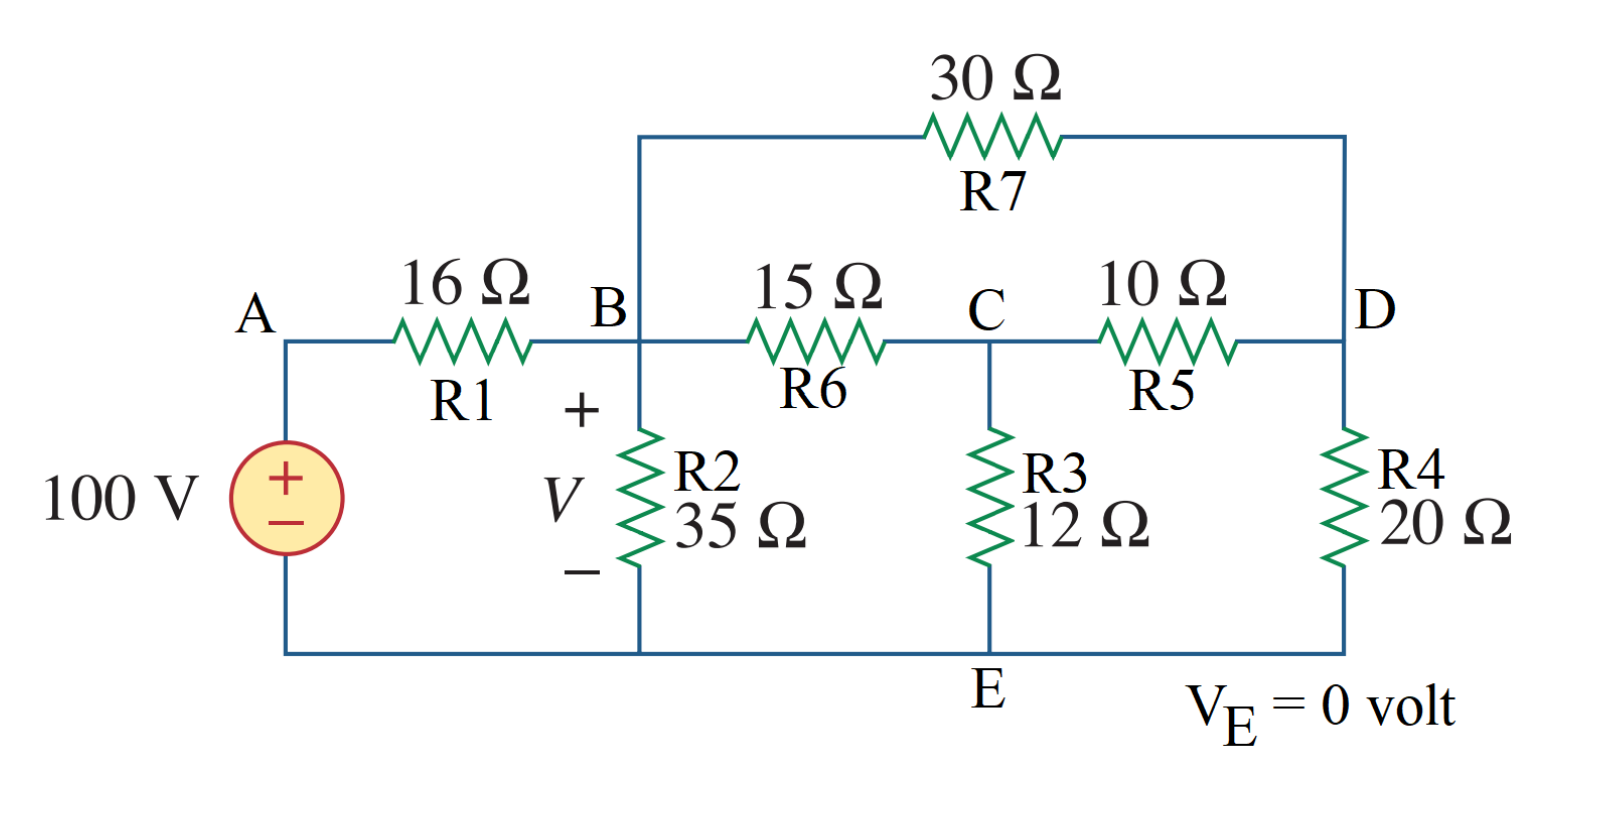
\includegraphics[scale=0.22]{graphics/ex10/f1.png}
    \caption{Mạch cấp nguồn chuyển mạch không hoàn chỉnh}
\end{figure}

\textbf{Tip:}

Để đặt bộ nguồn chuyển mạch IC LM2596 - 5.0, hãy vào \textbf{Place > PSpice Component...
> Search...} sau đó tìm kiếm LM2596\_5P0\_TRANS.

Nhưng trước khi bạn có thể thực hiện mô phỏng và phân tích nhất thời với mạch này, chúng ta sẽ
cần chú ý một số cài đặt nhỏ trên profile mô phỏng.

\begin{figure}[h]
    \centering
    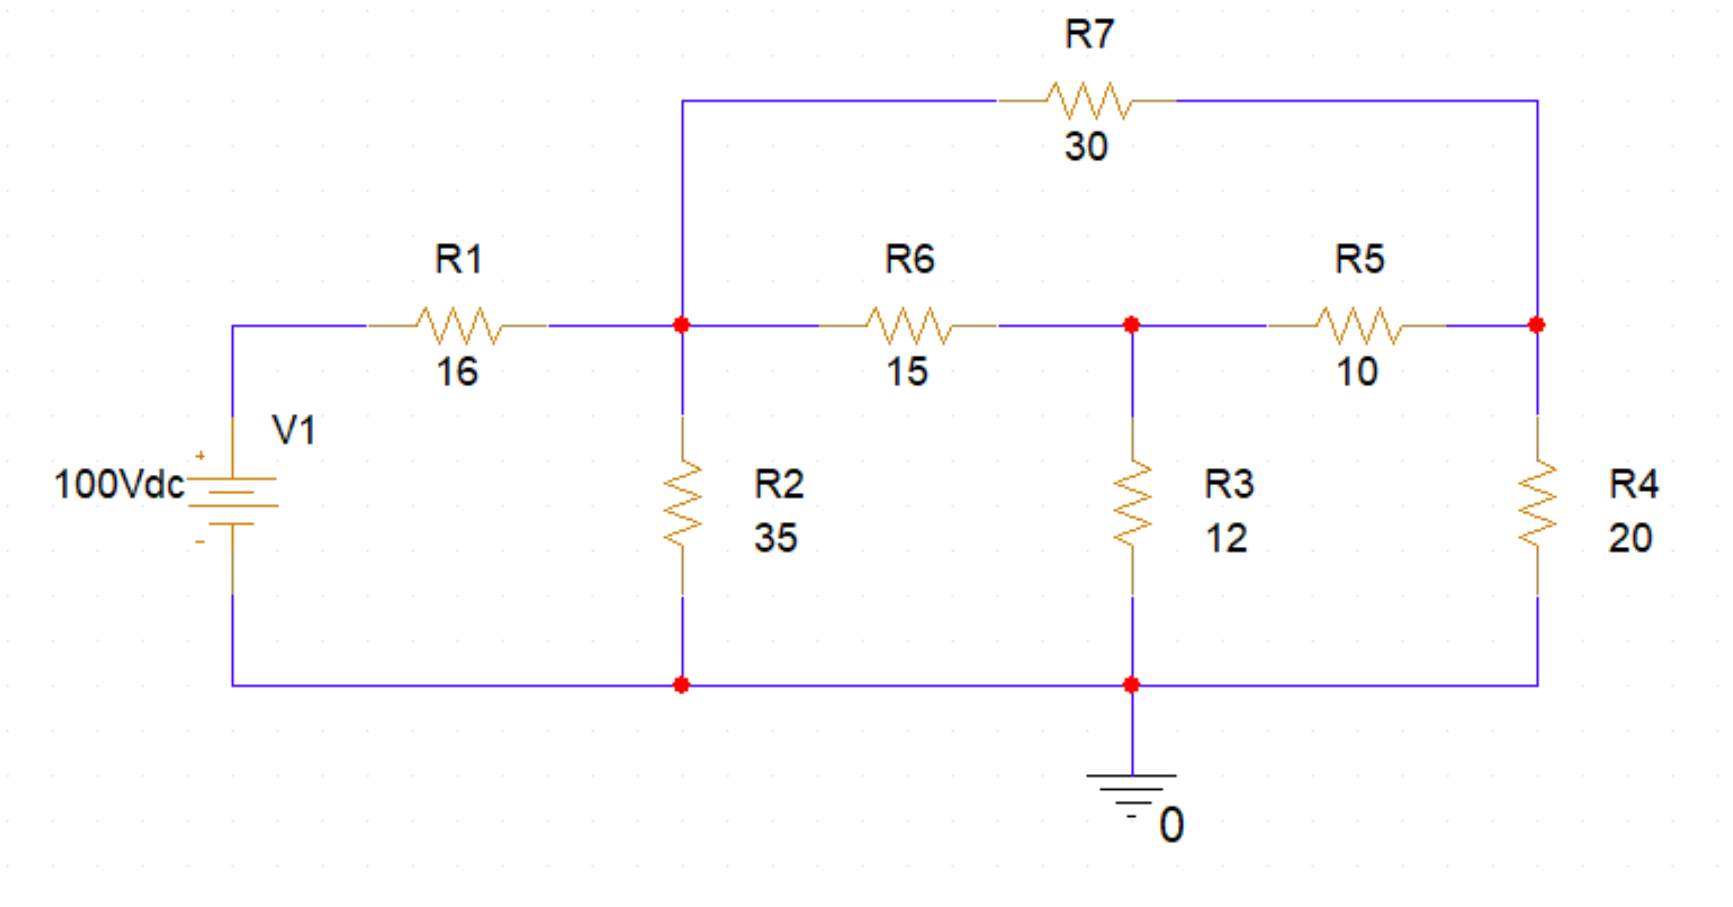
\includegraphics[scale=0.3]{graphics/ex10/f2.png}
    \caption{Đặt thời lượng mô phỏng nhất thời}
\end{figure}

\begin{figure}[ht]
    \centering
    \includegraphics[scale=0.3]{graphics/ex10/f3.png}
    \caption{Đặt độ chính xác tính toán nhất thời}
\end{figure}
\pagebreak
\textbf{Kết quả mô phỏng: }

\begin{figure}[ht]
    \centering
    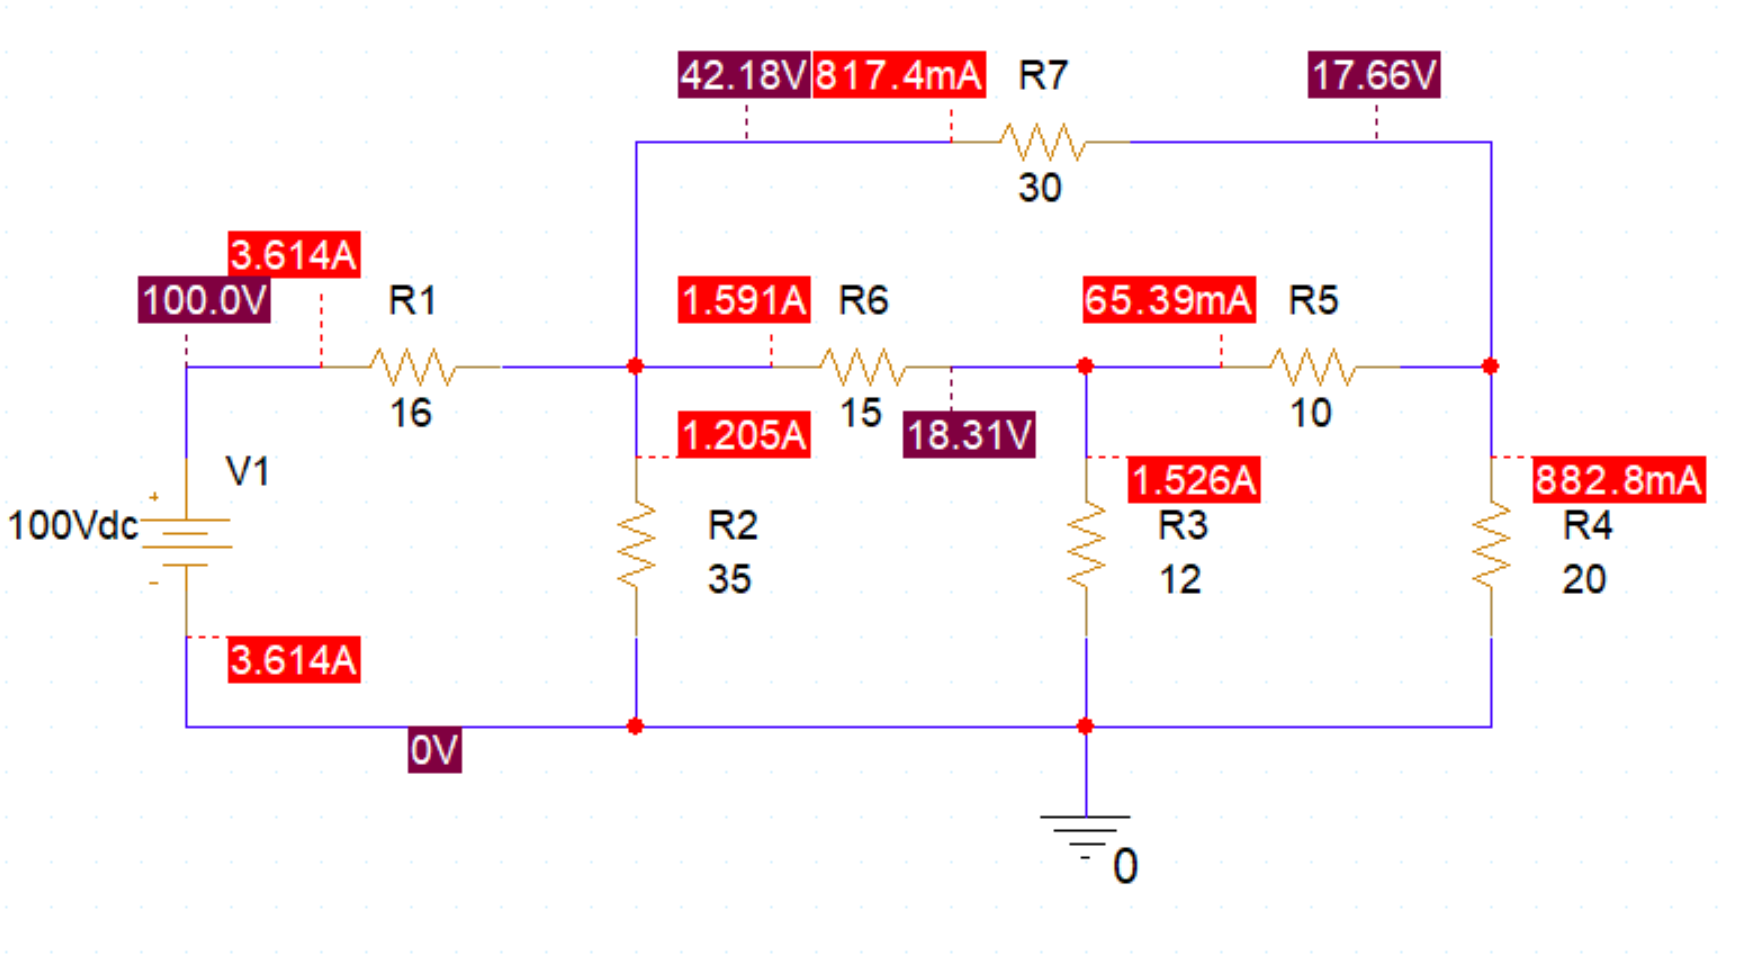
\includegraphics[scale=0.22]{graphics/ex10/f6.png}
    \caption{Kết quả mô phỏng của mạch trên}
\end{figure}

\textbf{Nhận xét và giải thích:} Đồ thị điện áp qua điện trở tăng nhanh trong khoảng 4ms đầu, sau đó giảm một chút rồi ổn định ở mức 5 (V) nhưng vẫn còn thay đổi một chút với sai số khoảng 0,03 (V).
\pagebreak

Tiếp theo, thêm một cuộn cảm 33µH vào mạch như trong Hình 10.5, sau đó chạy lại mô phỏng và giải thích mọi cải tiến.

\begin{figure}[ht]
    \centering
    \includegraphics[scale=0.23]{graphics/ex10/f4.png}
    \caption{Một cuộn cảm 33µH được thêm vào mạch}
\end{figure}

\textbf{Kết quả mô phỏng: }

\begin{figure}[ht]
    \centering
    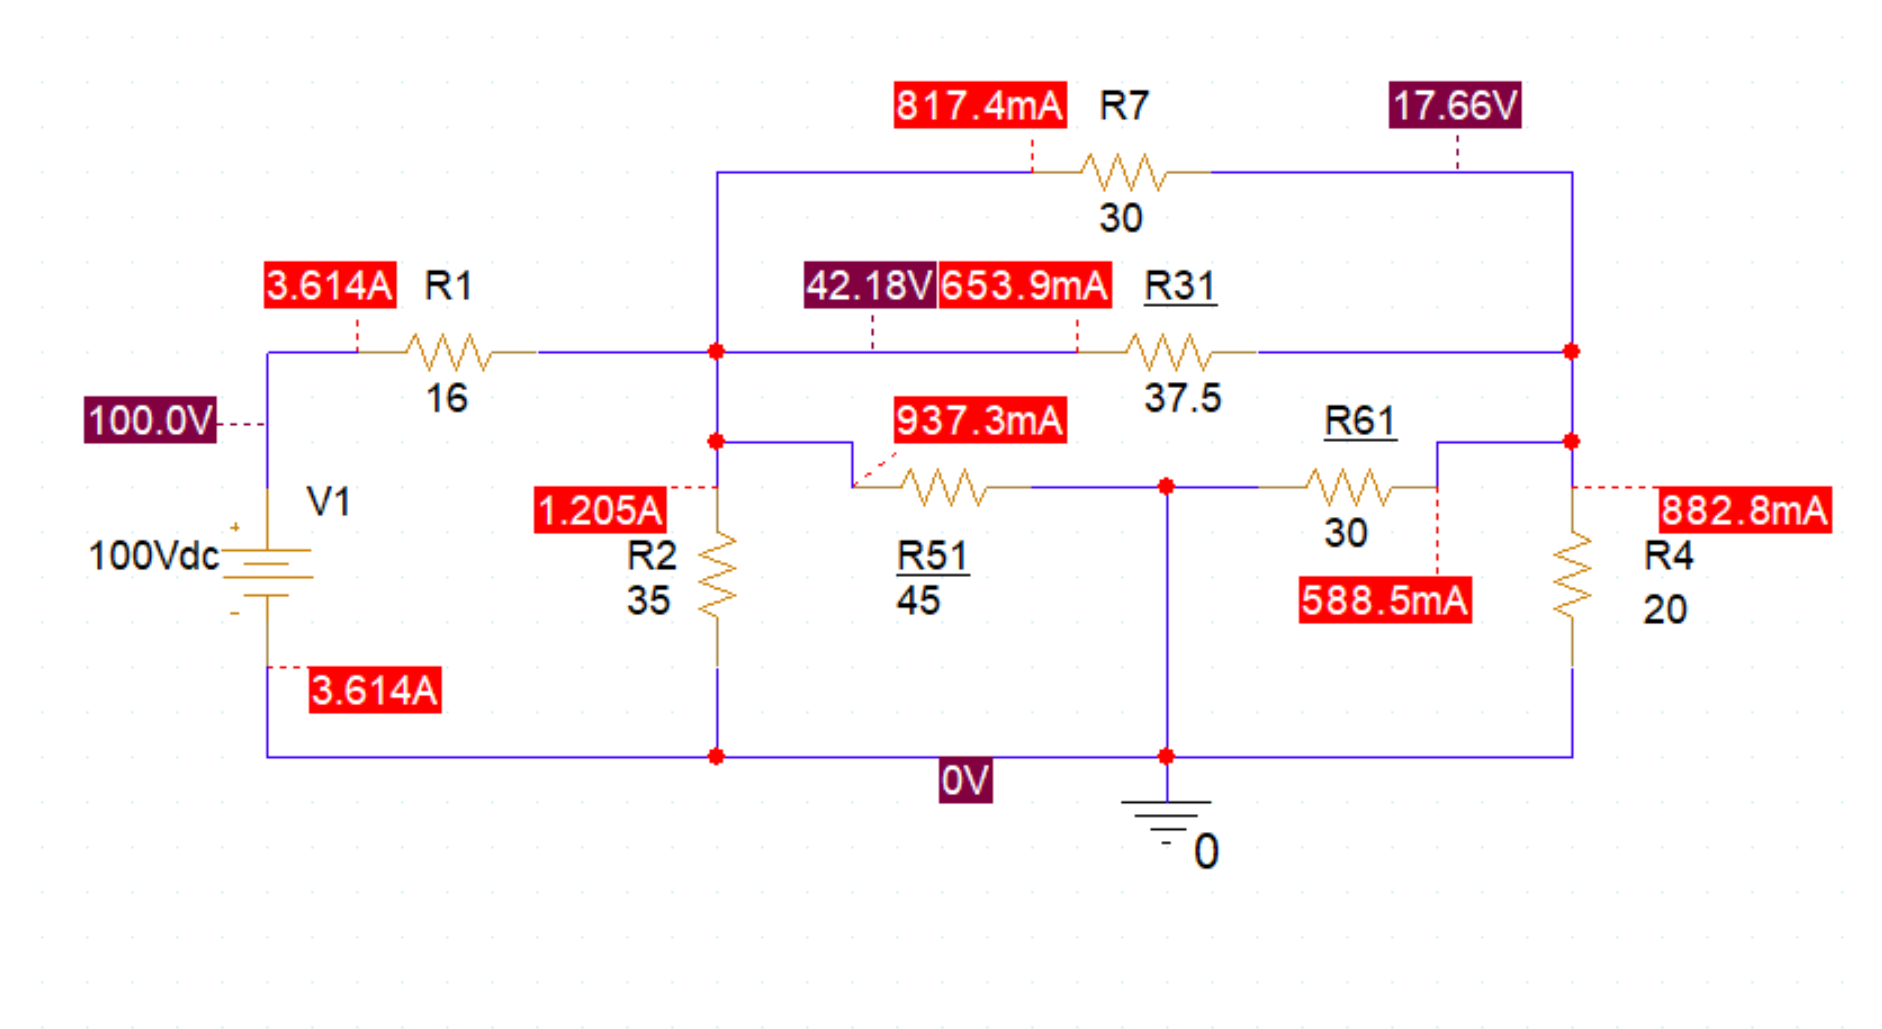
\includegraphics[scale=0.22]{graphics/ex10/f7.png}
    \caption{Kết quả mô phỏng của mạch trên}
\end{figure}

\textbf{Nhận xét và giải thích:} Đồ thị điện áp qua điện trở gần như không thay đổi trong 1ms đầu tiên, rồi tăng nhanh trong 1ms kế rồi ổn định ở mức điện áp 5 (V) nhưng còn chút gợn nhẹ với độ lệch khoảng 0,01 (V). Việc thêm cuộn cảm đã giúp cho mạch tăng điện áp nhanh hơn trong 2ms đầu và giúp cho điện áp ổn định hơn.
\pagebreak

Tiếp tục, thêm một diode Zener 5V vào mạch như hình 10.6, thay đổi tụ điện thành 220µF, thêm điểm đánh dấu dòng điện vào diode Zener, chạy lại mô phỏng và giải thích
vai trò của diode Zener trong mạch.

\begin{figure}[ht]
    \centering
    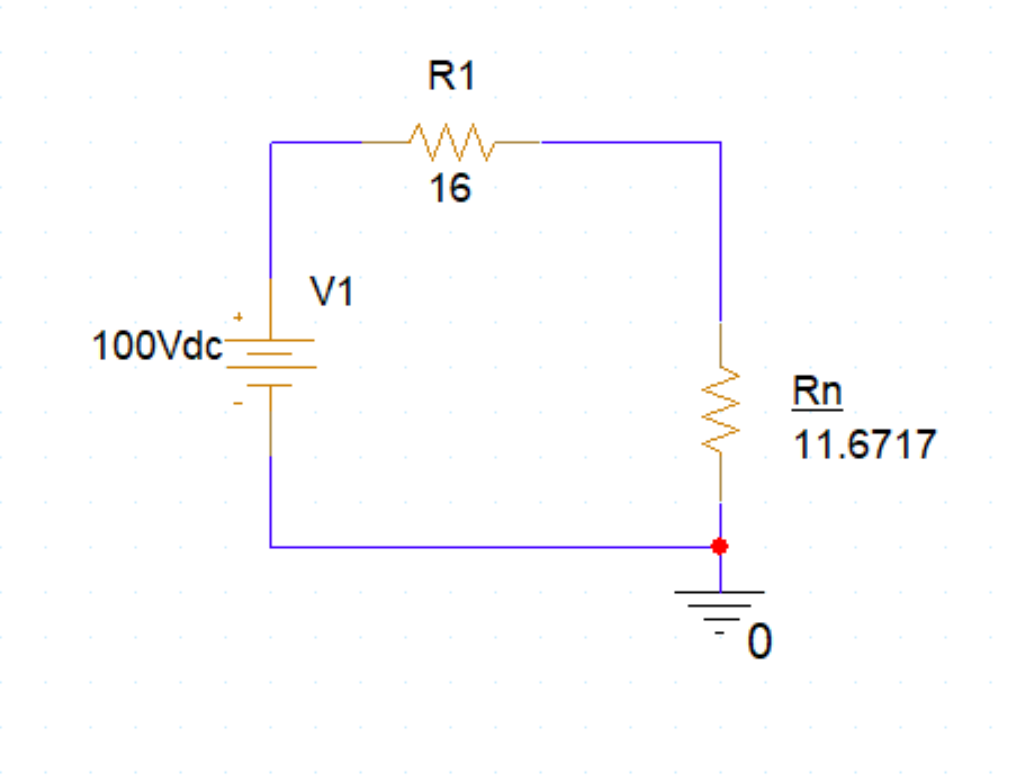
\includegraphics[scale=0.24]{graphics/ex10/f5.png}
    \caption{Một diode Zener 5V được thêm vào mạch}
\end{figure}

\textbf{Kết quả mô phỏng: }

\begin{figure}[ht]
    \centering
    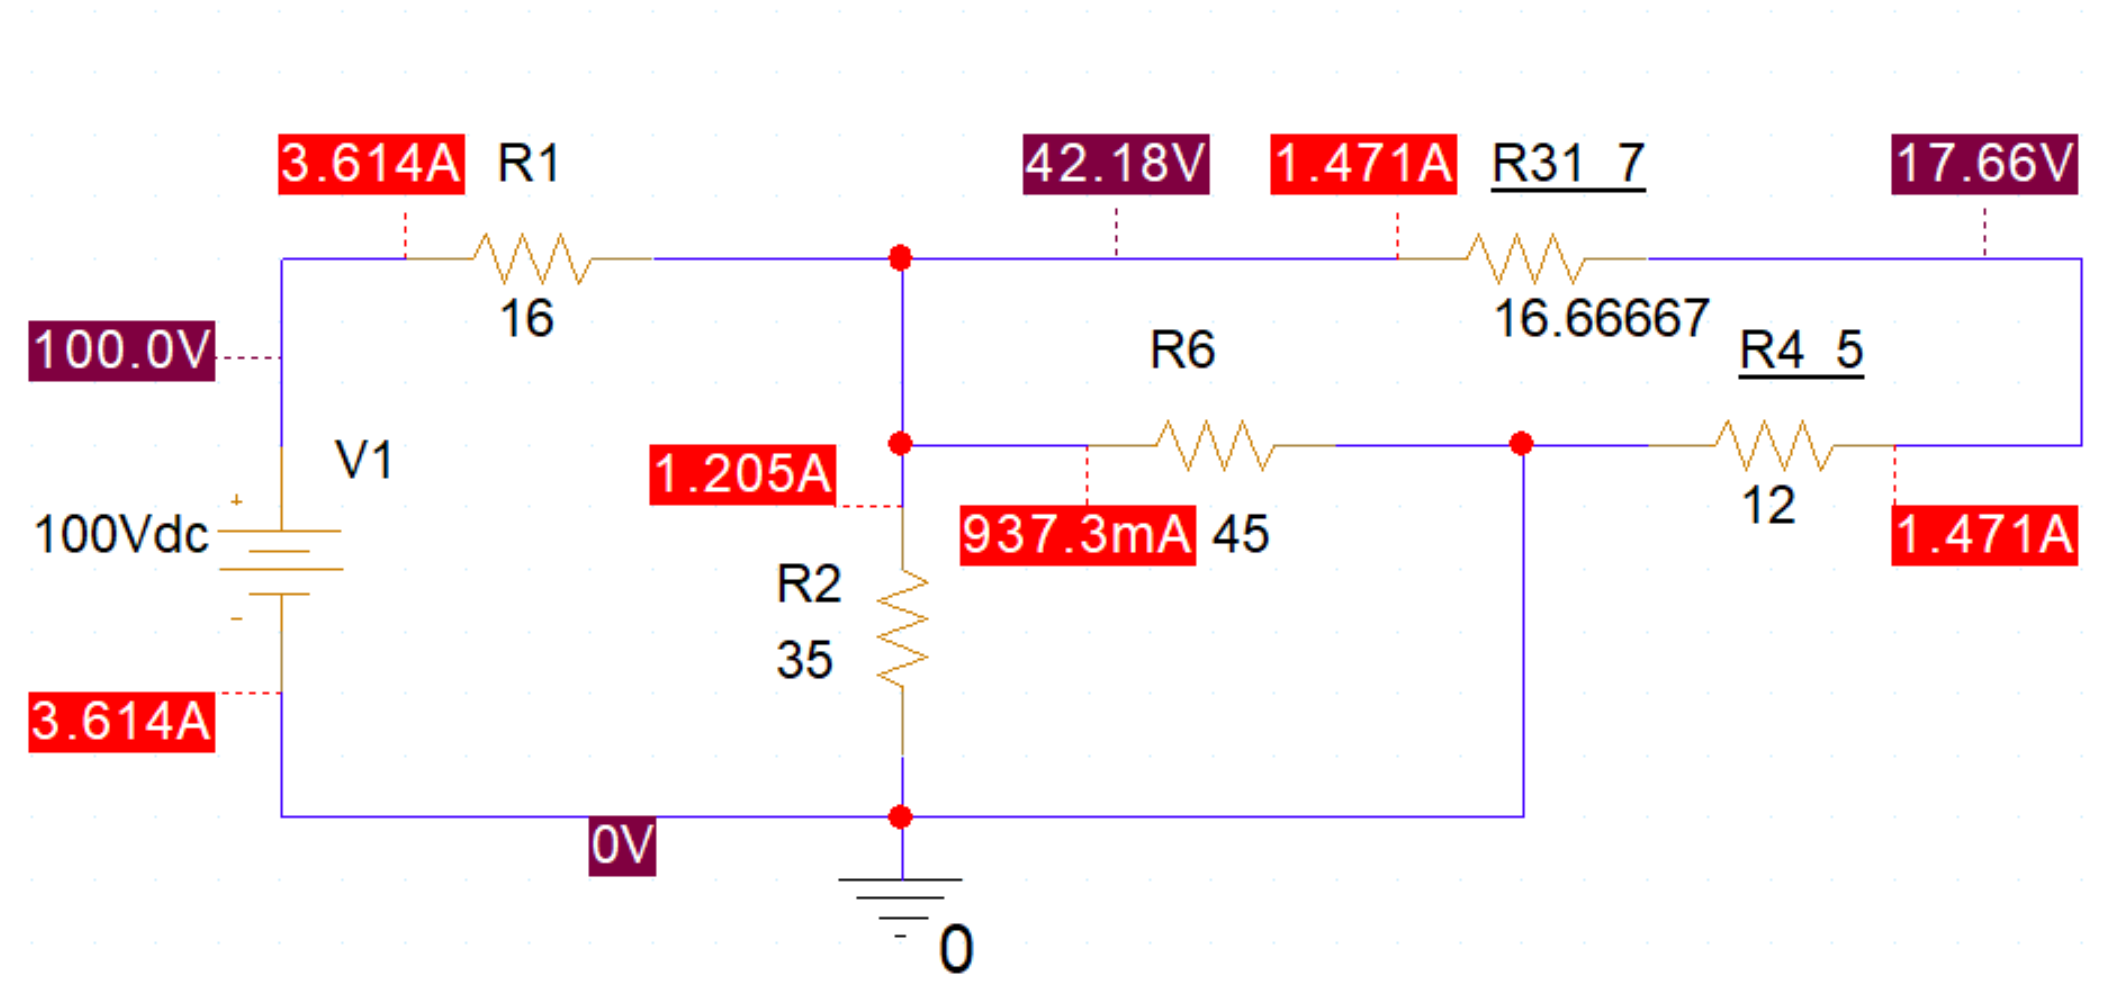
\includegraphics[scale=0.22]{graphics/ex10/f8.png}
    \caption{Kết quả mô phỏng của mạch trên}
\end{figure}

\textbf{Nhận xét và giải thích:} Đồ thị điện áp qua điện trở đã trở nên trơn hơn và ổn định hơn trước. Điều này là do việc thêm diode zener. Khi điện áp tại điện trở vượt qua 5(V), diode zener bắt đầu hoạt động và chống nhiễu, giúp điện áp luôn ổn định ở mức dưới 5 (V) (các gợn sóng màu đỏ trong hình biểu thị dòng điện tại diode khi điện áp tại điện trở vượt quá 5(V) ).





\end{document}